%% RSAA THESIS TEMPLATE, BY SIMON MURPHY <simon.murphy.nz@gmail.com>
%% BASED ON THE ORIGINAL TEMPLATE BY LATEX GOD JOSHUA RICH <joshua.rich@gmail.com>
%%
%% README:
% This template is designed to be used with pdflatex rather than plain
% latex.  It was developed under a TeXLive 2010 TeX distribution on
% a Mac, but should also work under Linux and earlier TeX distributions.
%
% For ANU requirements for typesetting and formatting see:
% http://policies.anu.edu.au/guidelines/research_theses_submission_and_examination___information_for_higher_degree_research_students/guideline

%%NOTES ABOUT THE DOCUMENT CLASS
% Yes, I'm using a report style.  Any 'thesis style' you might
% find or someone will give you is based on the standard report
% class, but is probably well outdated compared to whatever TeX
% you have installed.  Besides, why use that style file if you 
% have no idea what it actually does?  You will probably just redefine
% all of its customisations anyway...
\documentclass[a4paper,11pt,openright]{report} 
% ---------------------------------------------------------------------
% command re-definitions and additions
% ---------------------------------------------------------------------

% "Previously published as" chapter starter
\newcommand{\previouslypublished}[1]{\vspace{-0.5cm}\emph{\small #1}}

% i.e. -- e.g. -- etc. -- et. al.
\newcommand{\eg}{{\em e.g.,}}
\newcommand{\ie}{{\em i.e.,}}
\newcommand{\etc}{{\em etc.}}
\newcommand{\etal}{{\em et al.}}
\newcommand{\cf}{{\em cf.}}

% RESOLVE IVOA IDENTIFIERS TO THE US-VO DIRECTORY
% Use this to tag the particular dataset, VO service or tool you used in your research. Users can click on the link and resolve the full description in the US Virtual Observatory directory.
%
% e.g. "I used the NOMAD catalogue, as hosted by the Russian ASTRONET facility (\ivoa{ivo://astronet.ru/cas/nomad})"
%
\newcommand{\ivoa}[1]{\href{http://nvo.stsci.edu/vor10/getRecord.aspx?id=#1}{#1}}

% RESOLVE OBJECTS ON SIMBAD
% Adapted from http://tex.stackexchange.com/questions/4154/how-to-use-newcommand-for-href
% Same functionality as AASTEX macro: http://aastex.aas.org/objects/objectlinking.aas.htm
% #2 is mandatory object name (as written in the text) e.g. \object{IC 2391}
% #1 is optional SIMBAD name (if different from #2) e.g. \object[ETA CHA]{$\eta$~Cha}
\makeatletter
\newcommand{\object}[2][\simbadname]{%
\hypersetup{urlbordercolor=\objectcolor}%
\def\simbadname{#2}%
\StrSubstitute{#1}{ }{+}[\parsedname]%
\href{http://simbad.u-strasbg.fr/simbad/sim-id?Ident=\parsedname}{#2}%
\hypersetup{urlbordercolor=\urlcolor}}%
\makeatother

%% astronomical symbols
\newcommand{\HI}{\hbox{\rmfamily H\,{\textsc i}}}
\newcommand{\HIfat}{\hbox{\rmfamily\bfseries H\,{\textsc i}}}
\newcommand{\HIsub}{\hbox{{\scriptsize H}\,{\tiny I}}}
\newcommand{\HII}{\hbox{\rmfamily H\,{\scshape ii}}}
\newcommand{\HIIsub}{\hbox{\scriptsize \rmfamily H\,{\scshape ii}}}
\newcommand{\Ha}{\hbox{\rmfamily H\,$\alpha$}}
\newcommand{\msun}{\hbox{$M_{\odot}$}}
\newcommand{\mjup}{\hbox{$M_{\rm Jup}$}}
\newcommand{\mhi}{\hbox{$M_{\HIsub}$}}
\newcommand{\lsun}{\hbox{$L_{\odot}$}}
\newcommand{\mlsun}{(M/L)_{\odot}}
\newcommand{\vexp}{\hbox{$V_{exp}$}}
\newcommand{\vhel}{\hbox{$V_{hel}$}}
\newcommand{\vdisp}{\hbox{$\sigma_{disp}$}}
\newcommand{\Nhi}{\hbox{$N_{\HIsub}$}}
\newcommand{\nhi}{\hbox{$n_{\HIsub}$}}
\newcommand{\Mhi}{\hbox{$M_{\HIsub}$}}
\newcommand{\ra}{$\alpha$}
\newcommand{\dec}{$\delta$}
\newcommand{\degree}{\textdegree}
\newcommand{\arcmin}{\hbox{$^\prime$}}
\newcommand{\arcsec}{\hbox{$^{\prime\prime}$}}
\newcommand{\kms}{\hbox{km s$^{-1}$}}
\newcommand{\mjbeam}{\hbox{mJy beam$^{-1}$}}
\newcommand{\jbeam}{\hbox{Jy beam$^{-1}$}}
\newcommand{\mjbeamkms}{\hbox{mJy/beam km s$^{-1}$}}
\newcommand{\jkms}{\hbox{Jy km s$^{-1}$}}
\newcommand{\coldensity}{\hbox{cm$^{-2}$}}
\newcommand{\voldensity}{\hbox{cm$^{-3}$}}
% add others that you need, or can't be bothered writing repeatedly
\newcommand{\pms}{pre--main sequence}
\newcommand{\Pms}{Pre--main sequence}
\newcommand{\msunyr}{\hbox{$M_{\odot}$~yr$^{-1}$}}
\newcommand{\masyr}{mas~yr$^{-1}$}
\newcommand{\micron}{\hbox{$\mu$m}}
\newcommand{\wifes}{\hbox{\emph{WiFeS}}}
\newcommand{\vsini}{\ensuremath{v\sin i}}

% define any objects you will be referring to often
\newcommand{\echa}{\object[ETA CHA CLUSTER]{$\eta$~Cha}} 


% footnote symbols
% use \symbolfootnote[1]{footnote} to get an *
%     * 1 - *
%     * 2 - dagger
%     * 3 - double dagger
%     * 4 - ... 9 (see page 175 of the latex manual) 
\long\def\symbolfootnote[#1]#2{\begingroup%
\def\thefootnote{\fnsymbol{footnote}}\footnote[#1]{#2}\endgroup}
% New definition of square root:
% it renames \sqrt as \oldsqrt
% it defines the new \sqrt in terms of the old one
% See:
%  http://en.wikibooks.org/wiki/LaTeX/Tips_and_Tricks#New_Square_Root
\let\oldsqrt\sqrt
\def\sqrt{\mathpalette\DHLhksqrt}
\def\DHLhksqrt#1#2{%
\setbox0=\hbox{$#1\oldsqrt{#2\,}$}\dimen0=\ht0
\advance\dimen0-0.2\ht0
\setbox2=\hbox{\vrule height\ht0 depth -\dimen0}%
{\box0\lower0.4pt\box2}}

% define a new url command so a nice font can be used
\newcommand{\myurl}[1]{\href{#1}{#1}}

% ---------------------------------------------------------------------
% pdflatex setup
% ---------------------------------------------------------------------
% make pdflatex use the same spacing (paragraph, line and page breaks)
% as standard LaTeX 
\pdfadjustspacing=1

% ---------------------------------------------------------------------
%  misc. options
% ---------------------------------------------------------------------

% ---------------------------------------------------------------------
% more liberal 'float' (tables, figures) placement
% ---------------------------------------------------------------------
% Alter some LaTeX defaults for better treatment of figures:
% See p.105 of "TeX Unbound" for suggested values.
% See pp. 199-200 of Lamport's "LaTeX" book for details.
% General parameters, for ALL pages:
\renewcommand{\topfraction}{0.9}	% max fraction of floats at top
\renewcommand{\bottomfraction}{0.8}	% max fraction of floats at bottom
% Parameters for TEXT pages (not float pages):
\setcounter{topnumber}{2}
\setcounter{bottomnumber}{2}
\setcounter{totalnumber}{4}     % 2 may work better
\setcounter{dbltopnumber}{2}    % for 2-column pages
\renewcommand{\dbltopfraction}{0.9}	% fit big float above 2-col. text
\renewcommand{\textfraction}{0.07}	% allow minimal text w. figs
% Parameters for FLOAT pages (not text pages):
\renewcommand{\floatpagefraction}{0.7}	% require fuller float pages
% N.B.: floatpagefraction MUST be less than topfraction !!
\renewcommand{\dblfloatpagefraction}{0.7}	% require fuller float pages
% remember to use [htp] or [htpb] for placement

% ---------------------------------------------------------------------
% Journal name abbreviations
% ---------------------------------------------------------------------
\newcommand{\jnlref}[1]{\textrm{#1}}
\newcommand{\actaa}{\jnlref{Acta Astronomica}}
\newcommand{\aj}{\jnlref{AJ}}
\newcommand{\araa}{\jnlref{ARA\&A}}
\newcommand{\apj}{\jnlref{ApJ}}
\newcommand{\apjl}{\jnlref{ApJ}}
\newcommand{\apjs}{\jnlref{ApJS}}
\newcommand{\ao}{\jnlref{Appl.~Opt.}}
\newcommand{\apss}{\jnlref{Ap\&SS}}
\newcommand{\aap}{\jnlref{A\&A}}
\newcommand{\aapr}{\jnlref{A\&A~Rev.}}
\newcommand{\aaps}{\jnlref{A\&AS}}
\newcommand{\azh}{\jnlref{AZh}}
\newcommand{\baas}{\jnlref{BAAS}}
\newcommand{\jrasc}{\jnlref{JRASC}}
\newcommand{\memras}{\jnlref{MmRAS}}
\newcommand{\mnras}{\jnlref{MNRAS}}
\newcommand{\pra}{\jnlref{Phys.~Rev.~A}}
\newcommand{\prb}{\jnlref{Phys.~Rev.~B}}
\newcommand{\prc}{\jnlref{Phys.~Rev.~C}}
\newcommand{\prd}{\jnlref{Phys.~Rev.~D}}
\newcommand{\pre}{\jnlref{Phys.~Rev.~E}}
\newcommand{\prl}{\jnlref{Phys.~Rev.~Lett.}}
\newcommand{\pasp}{\jnlref{PASP}}
\newcommand{\pasj}{\jnlref{PASJ}}
\newcommand{\qjras}{\jnlref{QJRAS}}
\newcommand{\skytel}{\jnlref{S\&T}}
\newcommand{\solphys}{\jnlref{Sol.~Phys.}}
\newcommand{\sovast}{\jnlref{Soviet~Ast.}}
\newcommand{\ssr}{\jnlref{Space~Sci.~Rev.}}
\newcommand{\zap}{\jnlref{ZAp}}
\newcommand{\nat}{\jnlref{Nature}}
\newcommand{\iaucirc}{\jnlref{IAU~Circ.}}
\newcommand{\aplett}{\jnlref{Astrophys.~Lett.}}
\newcommand{\apspr}{\jnlref{Astrophys.~Space~Phys.~Res.}}
\newcommand{\bain}{\jnlref{Bull.~Astron.~Inst.~Netherlands}}
\newcommand{\fcp}{\jnlref{Fund.~Cosmic~Phys.}}
\newcommand{\gca}{\jnlref{Geochim.~Cosmochim.~Acta}}
\newcommand{\grl}{\jnlref{Geophys.~Res.~Lett.}}
\newcommand{\jcp}{\jnlref{J.~Chem.~Phys.}}
\newcommand{\jgr}{\jnlref{J.~Geophys.~Res.}}
\newcommand{\jqsrt}{\jnlref{J.~Quant.~Spec.~Radiat.~Transf.}}
\newcommand{\memsai}{\jnlref{Mem.~Soc.~Astron.~Italiana}}
\newcommand{\nphysa}{\jnlref{Nucl.~Phys.~A}}
\newcommand{\physrep}{\jnlref{Phys.~Rep.}}
\newcommand{\physscr}{\jnlref{Phys.~Scr}}
\newcommand{\planss}{\jnlref{Planet.~Space~Sci.}}
\newcommand{\procspie}{\jnlref{Proc.~SPIE}}
\newcommand{\ieeesigprocm}{\jnlref{IEEE~Signal~Processing~Magazine}}
\newcommand{\icarus}{\jnlref{Icarus}}
\let\astap=\aap
\let\apjlett=\apjl
\let\apjsupp=\apjs
\let\applopt=\ao


% define some constants that can be used in various places to easily
% specify title, subjects, author etc.
\newcommand{\thesistitle}{An interesting, detailed thesis title that will catch the reader's eye and leave them mesmerised!}
\newcommand{\fullname}{Andrew Raithby Casey}
\newcommand{\shortname}{A. R. Casey}
\newcommand{\thesissubjects}{astronomy,astrophysics}
\newcommand{\thesisdate}{\today}
\newcommand{\fullthesisdate}{\today}
\newcommand{\resubmissiondate}{\today}

\usepackage[british]{babel}
% ---------------------------------------------------------------------
% page size and margins
% ---------------------------------------------------------------------
%%NOTES ABOUT GEOMETRY PACKAGE:
% Below is using the geometry package as it is just cool.  This allows
% you to directly specify the margin requirements as outlined by ANU
% directly.  Here the inner border is 4cm and the outer is 2cm.  Top
% and bottom are also 2cm.  This is much easier than trying to work
% out page and margin dimensions by hand.  This is how you should use
% LaTeX...
\usepackage[pdftex]{geometry}
\geometry{a4paper,twoside}
\geometry{includehead}
\geometry{hmargin={3.8cm,2cm}}
\geometry{vmargin={1.6cm,1.9cm}}

% ---------------------------------------------------------------------
% miscellaneous packages used
% ---------------------------------------------------------------------
\usepackage{graphicx}
\usepackage{captcont}
\usepackage{array} % for setting line spacing in tables
\usepackage{epigraph}
\DeclareGraphicsExtensions{.pdf}
%\DeclareGraphicsExtensions{.eps}
\usepackage[twoside]{rotating}
\usepackage{ctable} % for good looking tables
\usepackage{xstring}
\usepackage[bottom]{footmisc}
\usepackage{pdflscape}
% fonts
\usepackage[T1]{fontenc}
\usepackage{textcomp}
\usepackage{ucs}
\usepackage[utf8x]{inputenc}
\usepackage{amsmath,amssymb}
\usepackage{pxfonts}
\usepackage{tgheros,tgpagella}
\renewcommand*\ttdefault{qcr}
\linespread{1.15} % tgpagella/mathpazo need a bigger line spacing
\usepackage{microtype}
%%NOTES ABOUT CAPTION AND SUBFIG PACKAGES
% I'm using the caption package to style my captions.
% You need to read the documentation for this package (on CTAN) as it
% has simple explanations of the options and examples of what it looks
% like.
%
% The subfig package allows the ability to control in detail
% positioning of sub-plots in a complex figure as well as add labels
% to them, which can then be referenced in the text without the need
% for changing the actual number as your sub-figures change.
% The subfig package inherits options from the caption package, so
% declare them together.
%
\usepackage[]{caption,subfig}
\DeclareCaptionLabelSeparator{mysep}{\ \ \ }
\captionsetup{format=plain,%
  indention=0cm,%
  labelsep=mysep,%
  justification=justified,
  labelfont={footnotesize,bf},%
  textfont={footnotesize}}
% bibliography uses natbib, this will be a requirement
\usepackage[round]{natbib}
% The hyperref package is a must while editing.  It provides urls
% inside your document; you can then click to go to certain pages,
% figures or bibliography entries.
%
% DEFINE MY CUSTOM COLORS
%
% change these to black if you want your citations and links nice and plain
%
\newcommand{\citecolor}{orange}
\newcommand{\linkcolor}{red}
\newcommand{\urlcolor}{blue}
\newcommand{\objectcolor}{gray}
%
\usepackage[hyperref,x11names]{xcolor}
\usepackage[unicode,pageanchor,colorlinks=true,plainpages=false,pdfpagelabels,pdftex]{hyperref}
\hypersetup{pdftitle=\thesistitle,%
  pdfauthor=\shortname,%
  pdfsubject={\thesissubjects},%
  citebordercolor=\citecolor,%
  linkbordercolor=\linkcolor,%
  urlbordercolor=\urlcolor,%
  citecolor=\citecolor,%
  linkcolor=\linkcolor,%
  urlcolor=\urlcolor%
}
% Stops figures and tables 'floating' past the section in which they
% are declared.
\usepackage[section]{placeins}
\usepackage[titletoc]{appendix}

\usepackage{ifthen}
\usepackage{xifthen}
% ---------------------------------------------------------------------
% styles for header, footer, pages, bibliography
% ---------------------------------------------------------------------
%

% chapter heading style
% this is the 'Conny' style from the fncychap package, modified to
% remove the two bold lines before the 'Chapter X' title.
% For usage of this package, see:
%  http://tug.ctan.org/cgi-bin/ctanPackageInformation.py?id=fncychap
%
\usepackage{fncychap}
\makeatletter
\ChNameUpperCase
% uncomment line below to convert all your chapter titles to CAPS
%\ChTitleUpperCase  
\ChNameVar{\centering\Huge\usefont{OT1}{qbk}{m}{n}\selectfont}
\ChNumVar{\Huge}
\ChTitleVar{\centering\Huge\usefont{OT1}{qbk}{m}{n}\selectfont}
\ChRuleWidth{2pt}
\renewcommand{\DOCH}{%
  \CNV\FmN{\@chapapp}\space \CNoV\thechapter
  \par\nobreak
  \vskip -0.5\baselineskip
}
\renewcommand{\DOTI}[1]{%
  \mghrulefill{\RW}\par\nobreak
  \CTV\FmTi{#1}\par\nobreak
  \vskip 60\p@
}
\renewcommand{\DOTIS}[1]{%
  \mghrulefill{\RW}\par\nobreak
  \CTV\FmTi{#1}\par\nobreak
  \vskip 60\p@
}

%
%%% page styles:
%
\usepackage{fancyhdr}
\pagestyle{fancy}
\renewcommand{\chaptermark}[1]{\markboth{#1}{}} 
\renewcommand{\sectionmark}[1]{\markright{\thesection\hspace{3mm} #1}{}} 
% redefine plain page style
\fancypagestyle{plain}{
\fancyhf{}
\fancyhead[LE]{\usefont{OT1}{qbk}{m}{n}\selectfont \thepage}
\fancyhead[RO]{\usefont{OT1}{qbk}{m}{n}\selectfont \thepage}
\renewcommand{\headrulewidth}{0pt}
\renewcommand{\footrulewidth}{0pt}
}

%
% this next section (till \makeatother) makes sure that blank pages
% are actually completely blank, cause they're not usually
\makeatletter
\def\cleardoublepage{\clearpage\if@twoside \ifodd\c@page\else
	\hbox{}
	\vspace*{\fill}
	\thispagestyle{empty}
	\newpage
	\if@twocolumn\hbox{}\newpage\fi\fi\fi}
\makeatother

%
%%% section header styles:
%
\usepackage[calcwidth]{titlesec}
\titlelabel{\thetitle.\quad}

% uncomment if you would like an index (make sure you actually define
% index terms in your document as well...
%\makeindex

% this contains various command definitions and other misc. options
\citestyle{aa}
\begin{document}
% epigraph settings, for quotes at the start of introduction and conclusions
\setlength{\epigraphwidth}{10cm}
\setlength{\afterepigraphskip}{1.5cm}
\renewcommand{\epigraphsize}{\small}
\renewcommand{\epigraphrule}{0pt}
\renewcommand{\epigraphflush}{center}
\renewcommand{\textflush}{flushleft}

% Andy: Had to comment out this line otherwise I was getting 
% 'can only be used in preamble' errors

\pagestyle{empty}

%
%%% TITLE PAGE:
%
% This title-page is based on many bits of information found on the
% Internet by searching for 'thesis title page latex'.  Packages are
% also available on CTAN if you don't like this style and don't feel
% confident creating a style yourself.
%
% Remove or change the \usefont..\selectfont if you don't have the
% TeX Gyre Bonum font.
%
\begin{titlepage}\usefont{OT1}{qbk}{m}{n}\selectfont
  \begin{center}
  \phantom{}
  \vspace{0cm}
    \huge{\thesistitle}
    \\[2.5cm]
    \huge{\fullname}
    \\[2.5cm]
    \LARGE{A thesis submitted for the degree of}\\[0.5cm]
      \LARGE{Doctor of Philosophy}\\[0.5cm]
      \LARGE{of the Australian National University}
    \\[3.cm]
     
\includegraphics[width=0.5\textwidth]{anu-logo-colour}
     \\[10mm]
        \LARGE{Research School of Astronomy \& Astrophysics}
        \vfill
        \Large{Submitted \thesisdate}\\[1mm]
% Uncomment this line when you print your final library copy        
%        \Large{Accepted \resubmissiondate}
  \end{center}
\end{titlepage}

\setlength{\parindent}{0pt}
\setlength{\parskip}{1ex plus 0.5ex minus 0.2ex}


% PREFACE TO ELECTRONIC COPY
% remember to change bib style file to "astroads" for the PDF copy
%%% COMMENT THIS OUT FOR THE PRINT COPY
\setcounter{page}{0} 
\phantomsection\addcontentsline{toc}{section}{Notes on the digital copy}
\setlength\fboxsep{3mm}
\setlength\fboxrule{1pt}
\begin{center}
\framebox{\huge{\textsc{Notes on the Digital Copy}}}
\end{center}
\vspace{5mm}
This document makes extensive use of the hyperlinking features of \LaTeX. References to figures, tables, sections, chapters and the literature can be navigated from within the PDF by clicking on the reference. Internet addresses will be displayed in a browser. 

Most object names are resolvable in the SIMBAD (\myurl{http://simbad.u-strasbg.fr/simbad/}) astronomical database. Click on an \object[NAME ETA CHA CLUSTER]{object} to be taken to its SIMBAD entry.

The bibliography at the end of this thesis has been hyperlinked to the NASA Astrophysics Data Service (\myurl{http://www.adsabs.harvard.edu/}). Further information on each of the cited works is available through the link to ADS.

Several of the large catalogues used in this work have been tagged with their Virtual Observatory unique identifier (e.g. \mbox{ivo://astronet.ru/cas/twomass-psc}). As~various data centres can have different versions and implementations of the same catalogue, this ensures any analysis is repeatable by denoting the exact catalogue \emph{and} service that was used to obtain the data. Clicking on their identifiers will resolve the service descriptions in the  directory hosted by the US Virtual Observatory (\myurl{http://ww.us-vo.org}).

\textbf{This page can be easily removed from the print copy\dots}

%%% END


 %
%%% DEDICATION:
%
% dedication page
\begin{figure}
\centering
{\large\usefont{OT1}{qzc}{m}{n}\selectfont 
To my cat, Mr Smigglesworth\dots
\\[4cm]\phantom{1}}
\end{figure}

\cleardoublepage
\normalsize
%
%%% FRONT CONTENT:
%
% page numbering as roman numerals
% don't indent paragraphs 
% increase the amount of space between paragraphs
\pagestyle{plain}
\pagenumbering{roman}
%
% disclaimer
%
% I don't like things showing up in the contents BEFORE the contents
% page itself, but you may wish to uncomment these lines.
%
%\phantomsection\addcontentsline{toc}{section}{Disclaimer}
\section*{Disclaimer}

I hereby declare that the work in this thesis is that of the candidate
alone, except where indicated below or in the text of the thesis. The work was undertaken between February 2010 and July 2013 at the Australian National University, Canberra, except for the period between July 2012 and December 2012 where the work was undertaken at the Massachusetts Institute of Technology, Boston. It has not been submitted in whole or in part for any other degree at this or any other university. 



\vspace{1cm}
\begin{flushright}

\includegraphics[width=0.4\linewidth]{signature.png}\\[2mm]
\fullname

\fullthesisdate
\end{flushright}


%
% acknowledgements
% \phantomsection\addcontentsline{toc}{section}{Acknowledgments}
\cleardoublepage
\section*{Acknowledgments}

Lorem ipsum dolor sit amet, consectetur adipiscing elit. Phasellus imperdiet volutpat turpis, vel aliquet elit tincidunt eu. Praesent convallis dolor ut tortor consectetur tincidunt. Nam ac molestie velit. Morbi luctus scelerisque purus id luctus. Fusce mattis risus eu sapien imperdiet tincidunt. Praesent laoreet blandit scelerisque. Suspendisse nec lorem velit. Nam scelerisque laoreet elementum. Sed justo urna, dapibus at varius eu, suscipit quis nibh. Integer lacinia, est sit amet accumsan luctus, nisl quam consectetur turpis, non tincidunt est ligula id sapien. Donec orci dui, convallis ac feugiat et, facilisis et velit. Donec ipsum ante, lobortis vitae auctor ac, sollicitudin a nisl. Aliquam leo leo, rhoncus ut sollicitudin et, euismod id ipsum. In in risus urna. Sed et nulla nibh, sed faucibus sem.

Maecenas est arcu, scelerisque a dapibus quis, molestie a mauris. Vestibulum egestas purus eget eros mollis placerat. Nulla porttitor, justo nec tincidunt hendrerit, nulla massa adipiscing ligula, feugiat tristique dui libero eget dolor. Phasellus id arcu id nisi faucibus eleifend vel a lacus. Vestibulum at elit eu neque vehicula elementum. Mauris bibendum massa nec urna rhoncus tempor. Curabitur in libero vitae quam vestibulum facilisis quis vitae velit. Donec tincidunt, lacus eget elementum sollicitudin, urna urna consequat ipsum, id eleifend eros augue at dolor. Praesent pellentesque, ante quis malesuada molestie, tortor lorem eleifend ante, sed rutrum massa dolor in lorem. Donec tempus, tellus eu fermentum ornare, sapien tortor tristique eros, quis blandit erat tortor eu lorem. Donec id tempus lectus. Donec ac odio eu elit molestie iaculis ac sed enim. Suspendisse et purus sem, convallis luctus mauris.

Duis massa mauris, sagittis vel dignissim non, rutrum ac nisi. Fusce ultricies mollis leo sit amet sagittis. Quisque lacinia placerat blandit. Vivamus est magna, tristique sed adipiscing in, sagittis sit amet dolor. Maecenas et nunc ipsum, in rutrum diam. Etiam ac nisl erat. Integer ac mi velit, in aliquam lacus. Etiam vitae nisi elit. Nam quam nisi, elementum eu porta eu, scelerisque vitae tortor. Nulla vel dolor magna. Aliquam suscipit, diam ac interdum pellentesque, tellus turpis sollicitudin nunc, vulputate congue massa massa vel urna. Sed a augue vel quam sollicitudin mollis.

Maecenas in lectus leo. Ut posuere lacus eget massa varius sit amet consectetur risus facilisis. Donec laoreet ornare pharetra. Maecenas vestibulum, lorem et suscipit vestibulum, enim lorem egestas eros, vitae vehicula orci sem sed dolor. Maecenas sit amet nibh nec lorem gravida hendrerit. Nulla tempus dui a lectus ornare vel viverra ipsum iaculis. Vestibulum ante ipsum primis in faucibus orci luctus et ultrices posuere cubilia Curae; Aliquam erat volutpat. In hac habitasse platea dictumst. Aenean dictum quam quis nunc tristique vitae blandit mauris dapibus. Sed velit tellus, adipiscing vitae commodo sit amet, lobortis eu orci. Morbi auctor mi eget sapien aliquet vel iaculis odio feugiat. Fusce semper risus suscipit ligula malesuada quis pretium diam rutrum. Donec varius nisi sit amet arcu interdum eu venenatis metus faucibus. 

%
% abstract
%\phantomsection\addcontentsline{toc}{section}{Abstract}
\cleardoublepage
\section*{Abstract}
Lorem ipsum dolor sit amet, consectetur adipiscing elit. Donec ac neque metus. Quisque a elit non justo pharetra lacinia at in dolor. Phasellus mauris mauris, sagittis id dapibus ac, facilisis vitae erat. Sed non urna mauris, nec rutrum nunc. Phasellus luctus metus nec diam hendrerit facilisis. Nulla metus ipsum, cursus in rutrum vel, rutrum ac risus. Vivamus feugiat bibendum lorem, quis iaculis nisi pellentesque at. Pellentesque fermentum tellus id lacus pharetra bibendum. Vestibulum luctus, lorem eget facilisis adipiscing, purus arcu fringilla diam, vel commodo lectus tellus non urna. Nulla elit nibh, sagittis at egestas ac, semper a elit. Nam sed dapibus sem. Mauris aliquam nulla quis arcu tincidunt auctor.

Mauris iaculis consequat porta. Quisque augue purus, auctor nec dapibus et, sodales quis nulla. Donec ipsum urna, mattis vitae consequat sed, pharetra ac dolor. Morbi placerat turpis quis eros gravida sed cursus orci posuere. Suspendisse eu malesuada arcu. Quisque turpis ante, vulputate in blandit non, molestie non leo. Quisque id erat id libero cursus pellentesque vitae a lacus. Nullam arcu ligula, sagittis id adipiscing bibendum.

Curabitur mattis consequat rutrum. Fusce vel risus non ipsum ullamcorper condimentum in a turpis. Class aptent taciti sociosqu ad litora torquent per conubia nostra, per inceptos himenaeos. Aenean sit amet odio nec augue ultricies dignissim tincidunt vel orci. Ut posuere lacinia tortor, vitae semper felis malesuada sit amet. In hac habitasse platea dictumst. Morbi vitae massa in turpis tincidunt gravida.

Cum sociis natoque penatibus et magnis dis parturient montes, nascetur ridiculus mus. Donec sodales ante eros. Suspendisse malesuada feugiat lacus vitae tincidunt. Proin eleifend arcu eget eros posuere vitae suscipit mi fringilla. Ut varius, purus id dapibus fermentum, ipsum ipsum euismod orci, vitae imperdiet nulla ligula in felis. In odio metus, ultricies sit amet sollicitudin sit amet, tempus in tortor. Nam sed turpis nulla. Fusce augue lectus, iaculis a hendrerit at, semper quis lacus. Nulla vestibulum justo nisi. Fusce egestas laoreet diam, convallis interdum elit fermentum eget. Sed ac mauris in odio dictum scelerisque.

Morbi nibh dui, adipiscing ac laoreet ac, vulputate sed metus. Sed lobortis est non lacus pellentesque a elementum tellus blandit. Ut porta, enim a ultricies mollis, arcu eros scelerisque nunc, lobortis facilisis orci ante in ipsum. Ut varius, quam eu vehicula euismod, diam leo mattis elit, ut vestibulum massa arcu a nunc. Suspendisse eleifend quam ac orci tincidunt congue. Praesent sit amet luctus lectus. Etiam interdum euismod sapien, dictum commodo nunc dictum vitae. Etiam quis sapien a felis congue ornare. Sed vel tristique tellus. In hac habitasse platea dictumst. Morbi mollis erat vel magna blandit faucibus. Duis mollis vestibulum sapien auctor mollis. Proin diam lacus, vulputate at feugiat pulvinar, mollis nec ipsum. Fusce orci enim, sollicitudin vel congue eu, tristique in diam. Pellentesque diam tellus, varius sed faucibus in, tincidunt at quam.

Aliquam erat volutpat. Curabitur rhoncus vestibulum lacinia. Sed in sollicitudin lacus. Curabitur non sem nunc. Sed nec metus a orci fermentum suscipit eu in ipsum. Sed ac arcu sed ipsum consequat sodales. Pellentesque habitant morbi tristique senectus et netus et malesuada fames ac turpis egestas.
%
% table of contents, figures and tables
\setcounter{tocdepth}{1} % limit TOC to sections, i.e. 1.2, not the default 1.2.1
%\phantomsection\addcontentsline{toc}{section}{Contents}
\tableofcontents\cleardoublepage
\phantomsection\addcontentsline{toc}{section}{List of Figures}
\listoffigures\cleardoublepage
\phantomsection\addcontentsline{toc}{section}{List of Tables}
\listoftables\cleardoublepage

%
% quotation at the start of the thesis
%\include{quote}

%
%%% MAIN CONTENT:
%
% page numbering as numbers for content of thesis
\pagenumbering{arabic}
\pagestyle{fancy}
\fancyhead[LO]{\usefont{OT1}{qbk}{m}{n}\selectfont \rightmark}
\fancyhead[RE]{\usefont{OT1}{qbk}{m}{n}\selectfont \leftmark}
\fancyhead[LE]{\usefont{OT1}{qbk}{m}{n}\selectfont \thepage}
\fancyhead[RO]{\usefont{OT1}{qbk}{m}{n}\selectfont \thepage}
\fancyfoot{}
\renewcommand{\headrulewidth}{0.5pt}
\renewcommand{\footrulewidth}{0pt}

\chapter{Introduction}\label{introduction}

\epigraph{The labour of the astronomer in the present state of his art is much like that of one who should examine, grain by grain, the sands of the sea in the certainty that among them numerous grains must exist of extraordinary value\dots}{-- Sir John Herschel\footnotemark}

\footnotetext{\emph{Memoirs of the Royal Astronomical Society.} 1826, Vol.\ 2, p472}


\section{The first of many sections}

Lorem ipsum dolor sit amet, consectetur adipiscing elit. Duis posuere tellus eu quam pellentesque ut varius purus egestas. Nam hendrerit malesuada sapien, non molestie risus cursus at. Pellentesque habitant morbi tristique senectus et netus et malesuada fames ac turpis egestas. Sed dignissim sodales sem sed volutpat. Ut laoreet, ante sed dictum vestibulum, lacus sapien semper dui, nec rutrum velit justo eu enim. Fusce vehicula blandit ipsum, ac volutpat libero vestibulum in. Sed quis lacus mauris. Quisque congue elit in nisi lacinia ac condimentum eros pellentesque. Quisque et nisl odio, vitae eleifend neque. Oh look, a sneaky citation to my paper \citep[][of which I am a co-author]{Kastner12}.


Phasellus erat libero, lobortis vitae iaculis nec, congue et tortor. Donec tempus leo et nisl tincidunt porta. Nulla velit sapien, sollicitudin sit amet accumsan a, facilisis a est. Phasellus scelerisque convallis sapien, nec viverra dui tincidunt a. Nulla ligula velit, laoreet fringilla condimentum sed, euismod a est. Fusce leo sapien, rhoncus a ultricies nec, porttitor ut lectus. Sed vestibulum turpis risus, nec vestibulum diam. Morbi quis quam quis enim cursus aliquam scelerisque quis tellus. Pellentesque accumsan lectus cursus massa ultrices placerat. Nulla facilisi. Praesent fermentum erat in augue sagittis condimentum. Nullam posuere blandit urna a mollis. Cras malesuada lectus a turpis sollicitudin volutpat. Morbi semper, nisl vel mattis vehicula, sapien sapien adipiscing tortor, in accumsan tortor dolor non neque. Maecenas varius, nunc ut euismod volutpat, mauris ante faucibus magna.

\subsection{A subsection}

Vestibulum sed orci nec diam euismod vehicula vitae et mauris. Phasellus sagittis justo quis mauris adipiscing auctor. Suspendisse nibh erat, cursus vitae aliquam in, rutrum sed est. Nunc mollis quam quis velit vehicula fringilla. Quisque convallis, neque ut faucibus luctus, nisl ante porttitor ante, at venenatis lectus nulla sed augue. Quisque lacinia semper lacus, nec ultricies justo auctor vel. Aenean viverra aliquam est ac porttitor.

% THIS FIGURE USES THE \echa MACRO DEFINED IN macros.tex
\begin{figure}[t!]
\vspace{-4mm}
   \centering
   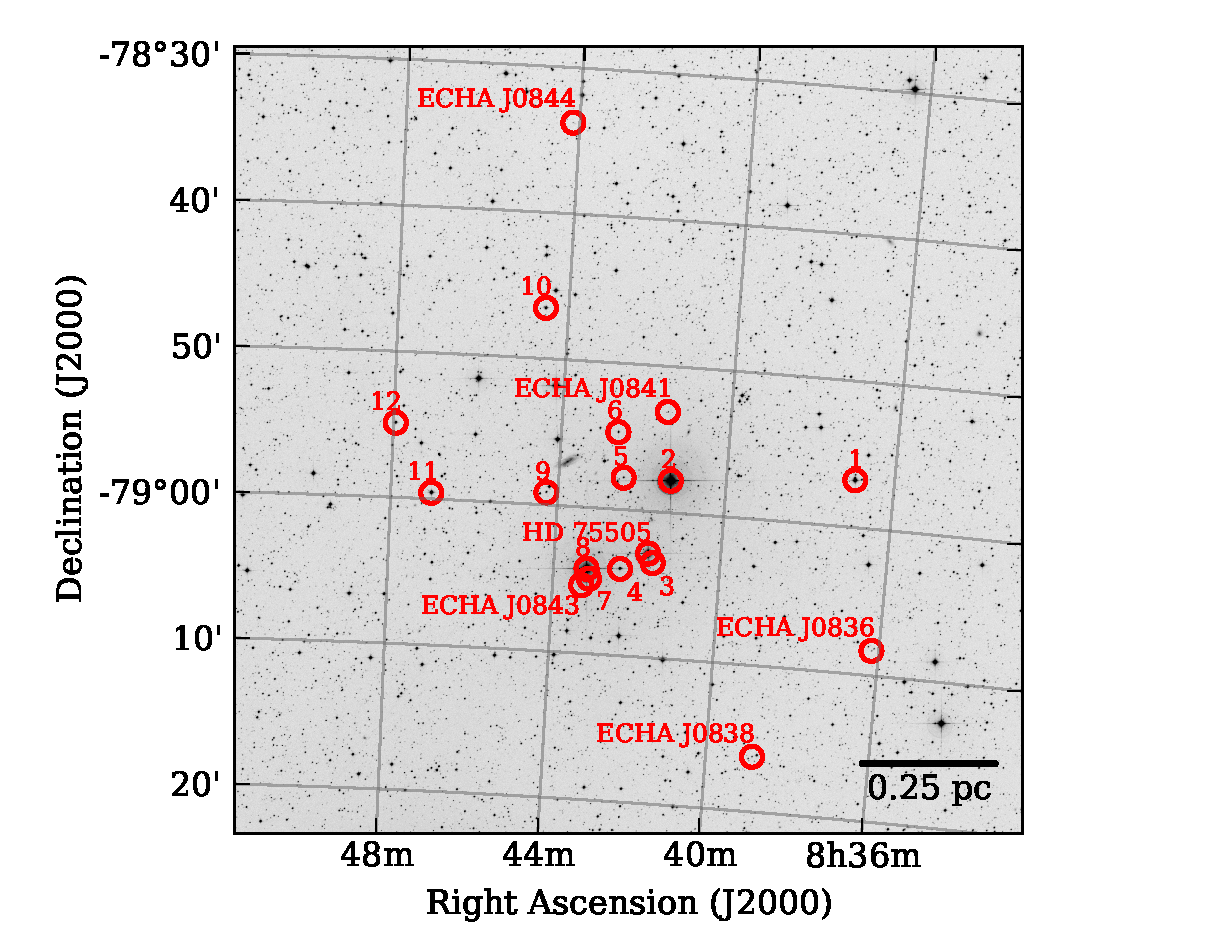
\includegraphics[width=\textwidth]{etacha} 
   \caption[{The \object[ETA CHA CLUSTER]{$\eta$ Chamaeleontis} open cluster}]{$0.9\times0.9$~deg DSS2-IR image showing the 18 member systems of the \echa\ cluster. The bright star at the centre of the image is the eponymous \echa. The bar shows the linear scale at the 94.3~pc cluster distance.}
   \label{fig:etacha}
\end{figure}

\section{Wow, another section heading!}

Sed tempor imperdiet rhoncus. Cras mi neque, pellentesque ac ultricies vitae, feugiat ut ante. Suspendisse vestibulum venenatis odio, quis pharetra mauris dapibus in. Pellentesque sagittis laoreet mi sed vestibulum. Ut iaculis venenatis urna eu tincidunt. Duis consequat est ut velit rutrum vitae placerat dolor eleifend. Nullam eget nulla massa, non accumsan libero. Sed auctor velit bibendum nisl tincidunt aliquam. Aenean pellentesque eros a lectus imperdiet rhoncus. Another citation to one of my papers \citep{Riedel11}.

Nunc non odio leo. Phasellus sodales pretium nunc suscipit bibendum. Nullam lorem turpis, varius sed bibendum id, interdum sed lectus. Ut rutrum, orci in adipiscing accumsan, velit massa dapibus metus, id volutpat nulla eros eget lorem. Ut massa massa, ornare vitae elementum ut, consequat a justo. Vestibulum tempus fermentum commodo. In vel auctor nisi. Mauris id turpis nisi. Nulla eget magna eu magna rhoncus pulvinar. Morbi enim ligula, feugiat et rutrum in, posuere eget lacus. Suspendisse adipiscing, erat in hendrerit dictum, est tellus vestibulum justo, et sodales mi dolor sed purus.

In porttitor purus et metus adipiscing molestie. Curabitur scelerisque, sem ac sodales sodales, neque metus commodo massa, eu pulvinar ante lectus eu orci. Mauris non odio vel enim scelerisque porttitor ac ac lacus. Pellentesque habitant morbi tristique senectus et netus et malesuada fames ac turpis egestas. Phasellus id dolor dui. Cras non neque vel turpis posuere commodo et nec leo. Nulla dictum rutrum nisi ac rhoncus. Aenean lobortis tempor magna viverra iaculis. Ut sit amet nunc mi. Integer iaculis condimentum diam non dignissim. Duis bibendum auctor velit id scelerisque.

Nulla tincidunt tortor ac odio posuere eget semper mauris tristique. Vestibulum congue magna sed arcu tincidunt id pharetra nisi hendrerit. Duis erat nulla, fringilla sed tempus at, sodales a libero. Nunc ullamcorper dapibus dui, ut varius tellus ullamcorper quis. Pellentesque odio lacus, molestie quis porta vitae, ornare eget massa. Integer hendrerit sapien ac massa lobortis in malesuada quam dignissim. Aliquam feugiat, nisl ut semper auctor, purus nunc iaculis ipsum, non tristique nibh felis a ipsum. Pellentesque odio lacus, molestie quis porta vitae, ornare eget massa. Ut sit amet nunc mi. Integer iaculis condimentum diam non dignissim. Duis bibendum auctor velit id scelerisque.

You can click on objects and be taken to their SIMBAD entry, like this: \object{Large Magellanic Cloud}. All of the objects in Table~\ref{table:etacha} are resolvable in SIMBAD.

% I think ctable gives the best LaTeX tables, once you get to know its syntax. All of the objects in this table are resolvable in SIMBAD using the \object{} command defined in macros.tex

\ctable[caption={Census of the \object[ETA CHA CLUSTER]{$\eta$ Chamaeleontis cluster} prior to this work},label=table:etacha,doinside=\small \setlength{\extrarowheight}{0pt}
,captionskip=0pt,pos=b]{lcccccccc}
{\tnote[$\dagger$]{\citet{Murphy10} (K and M members), \citet{Murphy11} (early-type members)}
\tnote[$\ddag$]{Photometry from \citet{Bessell12}}
\tnote[$\star$]{\object[ECHA J0844.2-7833]{ECHA J0844.2} has an elevated position in the cluster CMD}
}{
\toprule[2pt]
Name & Right Ascension & Declination & Spectral & $V$\tmark[$\ddag$] & Binary?\tmark[$\star$]\\
 & [J2000 deg] & [J2000 deg] & Type\tmark[$\dagger$] & [mag]\\
\midrule
 \object[ECHA J0836.2-7908]{ECHA J0836.2$-$7908} & 08 36 10.6 & $-$79 08 18 & M5.3 & 17.66 & suspected\\
  \object{RECX 1} & 08 36 56.2 & $-$78 56 46 & K7.0 & 10.61 & yes\\
  \object[ECHA J0838.9-7916]{ECHA J0838.9$-$7916} & 08 38 51.5 & $-$79 16 14 & M5.0 & 16.82 & suspected\\
  \object[ETA CHA]{$\eta$ Cha} (\object{RECX 2}) & 08 41 19.5 & $-$78 57 48 & B8V & 5.46& suspected\\
  \object[ECHA J0841.5-7853]{ECHA J0841.5$-$7853} & 08 41 30.6 & $-$78 53 07 & M4.7 & 17.07 & \\
  \object{RECX 3} & 08 41 37.2 & $-$79 03 31 & M3.0 & 14.35 \\
  \object{HD 75505} & 08 41 44.7 & $-$79 02 53 & A6 & 7.27\\
  \object{RECX 4} & 08 42 23.7 & $-$79 04 04 & M1.3 & 12.79\\
  \object{RECX 5} & 08 42 27.3 & $-$78 57 49 & M3.8 & 15.20\\
  \object{RECX 6} & 08 42 39.0 & $-$78 54 44 & M3.0 & 14.08\\
  \object{RECX 7} & 08 43 07.7 & $-$79 04 52 & K6.9 & 10.84 & yes\\
  \object{RS Cha} (\object{RECX 8}) & 08 43 12.2 & $-$79 04 12 & A8V+A8V & 6.28 & triple?\\
  \object[ECHA J0843.3-7905]{ECHA J0843.3$-$7905} & 08 43 18.4 & $-$79 05 21 & M3.4 & 13.97\\
  \object[ECHA J0844.2-7833]{ECHA J0844.2$-$7833} & 08 44 09.1 & $-$78 33 46 & M5.5 &  & suspected\\
  \object{RECX 9} & 08 44 16.6 & $-$78 59 09 & M4.4 & 15.00 & yes\\
  \object{RECX 10} & 08 44 32.2 & $-$78 46 32 & M0.3 & 12.53\\
  \object{RECX11} & 08 47 01.8 & $-$78 59 35 & K6.5 & 11.13\\
  \object{RECX 12} & 08 47 56.9 & $-$78 54 54 & M3.2 & 13.17 & suspected\\
\bottomrule[2pt]
}


chapter1/chapter1.tex
\chapter{Hunting the Parent of the Orphan Stream}

% you can put a brief note at the top of your chapters using '\previouslypublished{}'. For example, to give a reference to the paper this chapter is based on, or to point out that it has been submitted to a journal.

\previouslypublished{Parts of this chapter have been previously published as \href{http://adsabs.harvard.edu/abs/2013ApJ...764...39C}{`Hunting the Parent of the Orphan Stream: Identifying Stream Members from Low-Resolution Spectroscopy', {Casey}, A.~R., {Da Costa}, G., {Keller}, S.~C., {Maunder}, E., 2013, ApJ, 764, 39C}. The work is presented here in expanded and updated form.}

\section{Introduction}
We present candidate K-giant members in the Orphan Stream which have been identified from low-resolution data taken with the AAOmega spectrograph on the Anglo-Australian Telescope. From modest S/N spectra and independent cuts in photometry, kinematics, gravity and metallicity we yield self-consistent, highly probable stream members. We find a revised stream distance of $22.5\,\pm\,2.0$\,kpc near the celestial equator, and our kinematic signature peaks at $V_{GSR} = 82.1\,\pm\,1.4$\,km s$^{-1}$. The observed velocity dispersion of our most probable members is consistent with arising from the velocity uncertainties alone. This indicates that at least along this line-of-sight, the Orphan Stream is kinematically cold. Our data indicates an overall stream metallicity of [Fe/H] $= -1.63\,\pm\,0.19$\,dex which is more metal-rich than previously found and unbiased by spectral type. Furthermore, the significant metallicity dispersion displayed by our most probable members, $\sigma(\mbox{[Fe/H]}) = 0.56$\,dex, suggests that the unidentified Orphan Stream parent is a dSph satellite. We highlight likely members for high-resolution spectroscopic follow-up.
\end{abstract}

\keywords{Galaxy: halo, structure --- Individual: Orphan Stream --- Stars: K-giants}

\section{Introduction}
\label{sec:ch2-introduction}

The Milky Way stellar halo has partly formed through the accretion of satellites that are disrupted by tidal forces as they fall into the Galaxy's potential. Stars which were once gravitationally bound to the satellite are distributed along the progenitor's orbit in leading and trailing streams of stars. The velocities of stars in the stream are sensitive to the shape of the dark matter halo, allowing us to constrain the Milky Way potential and reconstruct the formation history of the Galaxy. The level of accreted substructure in the Milky Way has only recently become apparent through multi-band photometric surveys like the Sloan Digital Sky Survey (SDSS). The more prominent of the detectable substructures, like Sagittarius, have been well-studied. One of the more prominent \--- yet less studied \--- substructures is that of the Orphan Stream. 

% could add a sentence to the paragraph above discussing the various substructures that have been detected

The Orphan Stream was independently detected by both \citet{Grillmair_2006} and \citet{Belokurov_et-al_2006}, and is distinct from other substructures in the halo. The stream stretches over $60\,^\circ$ in the sky, has a low surface brightness, and a narrow stream width of only $\sim$2\,$^\circ$.  As the name suggests, the parent object largely remains a mystery. The stream extends past the celestial equator \--- outside the SDSS footprint \--- but has not been detected in existing southern surveys \citep{Newberg_et-al_2010}. Whilst the parent system remains elusive, significant effort has been placed on associating the stream with known Milky Way satellites \citep{Zucker_et-al_2006, Fellhaur_et-al_2007,Jin_Lynden_Bell_2007,Sales_et-al_2008}. In contrast, there has been relatively limited observational work on the Orphan Stream itself other than the original discovery papers \citep{Grillmair_2006, Belokurov_et-al_2006, Belokurov_et-al_2007} and the work of \citet{Newberg_et-al_2010}. This is largely to be expected given the absence of deep multi-band photometry in the southern sky and the low total luminosity of the stream. This makes it difficult to reliably separate Orphan Stream members from halo stars. Understanding the full extent of the stream awaits the SkyMapper and Pan-STARRS photometric surveys \citep{Keller_et-al_2007, Hodapp_et-al_2004}.

As \citet{Sales_et-al_2008} point out, there is a natural observational bias towards more massive and recent mergers like Sagittarius. Consequently, the fainter end of this substructure distribution has yet to be fully recovered, or thoroughly examined. Interestingly, there are indications that  some fainter substructures like the Orphan Stream and the Palomar 5 tidal tails \citep{Odenkirchen_et-al_2009} have orbits which seem to be best-fit by Milky Way models with nearly 60\% less mass \citep{Newberg_et-al_2010} than generally reported by \citet{Xue_et-al_2008} and \citet{Koposov_et-al_2010}. Such a discrepancy in the mass of the Milky Way is troublesome. More complete photometric and kinematic maps of these low total luminosity streams may provide the best test as to whether this mass discrepancy is real, or an artefact of incomplete observations. Whilst the full spatial extent of the Orphan Stream remains unknown, we can examine the detailed chemistry of its members, investigate the stream history, and make predictions about the nature of the progenitor.

In this paper we present a detailed, self-consistent analysis to identify K-giant members of the Orphan Stream. Using our selection method we have catalogued the locations of nine highly probable Orphan Stream candidates, all worthy of high-resolution spectroscopic follow up. In the following section we outline our photometric target selection. In \S\ref{sec:ch2-observations} we describe the low-resolution spectroscopic observations. The data analysis, including stream identification, is discussed in \S\ref{sec:ch2-analysis} and in \S\ref{sec:ch2-conclusions} the conclusions, predictions and future work are presented.


\section{Target Selection}
\label{sec:ch2-target-selection}

We have targeted K-giant members of the Orphan Stream in order to investigate their detailed chemistry. Because K-giants are difficult to unambiguously detect from photometry alone, low-resolution spectroscopy is required to estimate stellar parameters and determine radial velocities. The Orphan Stream has an extremely low spatial over-density, which makes it difficult to separate stream members from halo stars. However, there is a well described distance gradient along the stream \citep{Belokurov_et-al_2007, Newberg_et-al_2010} which provides an indication on where we should focus our spectroscopic efforts.

The Orphan Stream is closest to us in two locations on the edge of the SDSS footprint: at the celestial equator \citep{Belokurov_et-al_2007}, and along outrigger SEGUE Stripe 1540 \citep{Newberg_et-al_2010}. These two locations are unequivocally the best place to recover bright stream members. We have targeted two fields centered on $(\alpha, \delta) =$ (10:48:15, 00:00:00) and (10:48:15, $-$02:30:00), and employed a combination of colour cuts with the SDSS DR 7 \citep{Abazajian_et-al_2009} data set in order to identify likely K-giants:
\begin{eqnarray}
0.6 <& (g-i)_0 &< 1.7 \\
-15(g-i)_0 + 27 <& g_0 &< -3.75(g-i)_0 + 22.5 \\
15  <& i_0  &< 18 
\end{eqnarray}

Given our colour selection we expect to recover giants and contaminating dwarfs. Although the 2MASS $JHK$ colours can help to separate dwarfs and giants, our target K-giants stars are too faint to be detected in the 2MASS catalogue.

\section{Observations}
\label{sec:ch2-observations}

Observations took place on the Anglo-Australian Telescope using the AAOmega spectrograph in April 2009. AAOmega is a fibre-fed, dual beam multi-object spectrograph which is capable of simultaneously observing spectra of 392 (science and sky) targets across a $2\,^\circ$ field of view. We used the 5700\,{\AA} dichroic in combination with the 1000I grating in the red arm, and the 580V grating in the blue arm. This provides a spectral coverage between $800 \leq \lambda \leq 950$\,nm in the red at $\mathcal{R} \approx 4400$, and between $370 \leq \lambda \leq 580$\,nm with a lower spectral resolution of $\mathcal{R} \approx 1300$ in the blue.

The data were reduced using the standard \textsc{2DFDR} reduction pipeline\footnote{http://www.aao.gov.au/2df/aaomega/aaomega\_2dfdr.html}. After flat-fielding, throughput calibration for each fibre was achieved using the intensity of skylines in each fibre. The median flux of dedicated sky fibres was used for sky subtraction, and wavelength calibration was performed using ThAr arc lamp exposures taken between science frames. Three thirty minute science exposures were median-combined to assist with cosmic ray removal. The median S/N obtained in the red arm for our fields is modest at 35 per pixel, although this deteriorates quickly for our fainter targets. With the presence of strong Ca\,\textsc{II} triplet lines in the red arm we are able to ascertain reliable radial velocities and reasonable estimates on overall metallicity \citep[][and references therein]{Starkenburg_et-al_2010}. Our spectral region also includes gravity-sensitive magnesium lines: Mg\,\textsc{I} at 8807\,{\AA}, and the Mg\,\textsc{I}\,b 3$p$-4$s$ triplet lines at $\sim$5178\,{\AA}. As we demonstrate in the next section, these lines are sufficient to discriminate dwarfs from giants even with weak signal.

The blue and red arm spectra were normalised using a third order cubic spline after multiple iterations of outlier clipping. We used defined knot spacings of 20 nm in the red arm, and 5 nm in the blue arm in order to accommodate often poor S/N, and varying strengths of molecular band-heads.

\section{Analysis \& Discussion}
\label{sec:ch2-analysis}

We have employed a combination of separate criteria to identify likely Orphan Stream members: kinematics, a giant/dwarf indication from Mg\,\textsc{I} lines, and selecting stars with consistent metallicities derived from both isochrone fitting and the strength of the Ca\,\textsc{II} triplet lines. Each criteria is discussed here separately.

\subsection{Kinematics}
Radial velocities were measured by cross-correlating our normalised spectra against a K-giant synthetic template with a temperature of 4500\,K, $\log{g}$ = 1.5 and $[\mbox{M/H}] = -1.5$ across the range $845 \leq \lambda \leq 870$\,nm. Heliocentric velocities were translated to the galactic rest frame by adopting the local standard of rest velocity as 220\,km s$^{-1}$ towards $(l, b) = (53\,^\circ, 25\,^\circ)$ \citep{Kerr_Lynden-Bell_1986, Mihalas_Binney_1981}\footnote{Where $V_{GSR} = V_{HELIO} + 220\sin{l}\cos{b} + 16.5\times[\sin{b}\sin{25^\circ} + \cos{b}\cos{25^\circ}\cos{(l - 53^\circ)}]$}.

Figure \ref{fig:ch2-velocities} shows a histogram of our galactocentric velocities, compared to the predicted smooth line-of-sight velocity distribution for this region from the Besan\c{c}on model \citep{Robin_et-al_2003}. We have selected particles from the Besan\c{c}on model using the same criteria outlined in \S\ref{sec:ch2-target-selection} after employing the \citet{Jordi_et-al_2006} colour transformations. It is clear that our target selection has yielded mostly nearby disk dwarf stars with $V_{GSR} \approx -120$\,km s$^{-1}$.

\begin{figure}[h]
	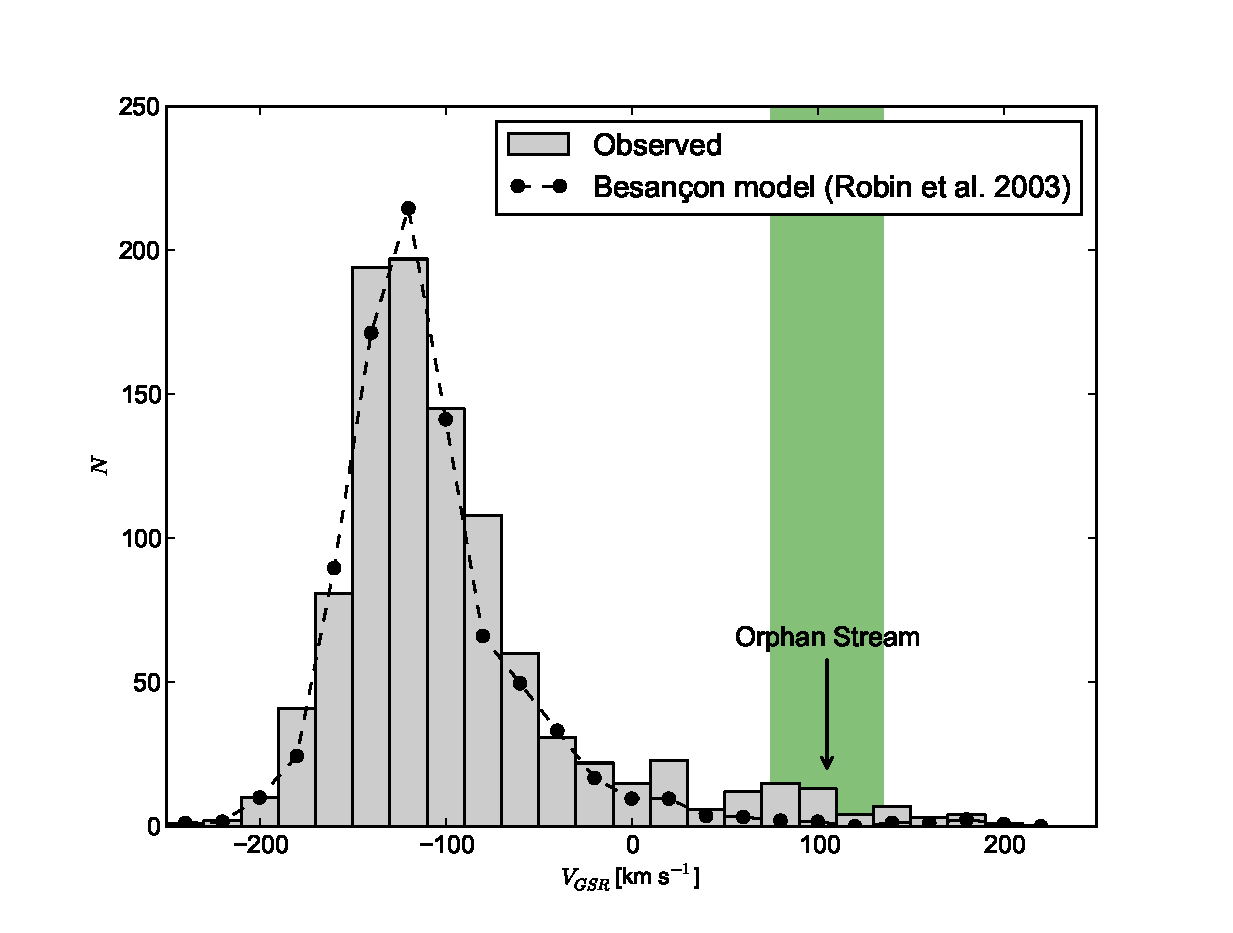
\includegraphics[width=\columnwidth]{./fig1.eps}
	\caption{Galactocentric rest frame velocities for stars in both our observed fields (grey), and predicted Besan\c{c}on velocities which have been scaled to match our observed sample size. The expected kinematic signature from \citet{Newberg_et-al_2010} for the Orphan Stream is highlighted, as is our kinematic selection window (green).}
	\label{fig:velocities}
\end{figure}
 

In a nearby ($\Delta\Lambda_{Orphan} \sim 4\,^\circ$) region of the stream, \citet{Newberg_et-al_2010} detected the Orphan Stream with a $V_{GSR} = 101.4$ km s$^{-1}$ from BHB stars. Differences in accounting for the local standard of rest between this work and \citet{Newberg_et-al_2010} means that this corresponds to approximately 95\,km s$^{-1}$ on our $V_{GSR}$ scale.  This is discussed further in \S\ref{sec:ch2-newberg}. The expected Orphan Stream kinematic peak is labelled in Figure \ref{fig:ch2-velocities}. There is no obvious sharp kinematic peak representative of the Orphan Stream in our sample. From kinematics alone, our targets appears largely indistinguishable from a smooth halo distribution. To isolate potential Orphan Stream members we have nominated a relatively wide selection criteria between $65 \leq V_{GSR} \leq 125$ km s$^{-1}$ (shown in Figure \ref{fig:ch2-velocities}), which yields 28 Orphan Stream candidates. The typical uncertainty in our velocities is $\pm{}5.0$\,km s$^{-1}$.

\subsection{Dwarf/Giant Discrimination}
\label{sec:ch2-dwarf-giant}

We have measured the equivalent width of the gravity-sensitive Mg\,\textsc{I} line at 8807 \AA{} to distinguish dwarfs from giants \citep{Battaglia_Starkenburg_2012}. At a given temperature (or $g - r$) and metallicity, giant stars present narrower Mg\,\textsc{I} absorption lines than their dwarf counterparts. Given the target selection, our sample is likely to contain many more dwarfs than giants (e.g. see \citet{Casey_et-al_2012} where a similar colour selection was employed). In some cases no Mg\,\textsc{I} 8807 \AA{} line was apparent, so an upper limit was estimated based on the S/N of the spectra. In these cases the candidate was considered a ``non-dwarf" because we cannot exclusively rule out a metal-poor sub-giant with this criteria alone. For these purposes we are only looking for a simple indication as to whether a star is likely a dwarf or not. 

Figure \ref{fig:ch2-ew-mg} illustrates the trend with $EW_{\lambda8807}$ against SDSS de-reddened\footnote{All magnitudes presented in this letter are de-reddened using the \citet{Schlegel_Finkbeiner_Davis_1998} dust maps.} $g - r$, illustrating the dominant upper dwarf branch we wish to exclude. Giant stars populate the lower, sparser branch. A separation line has been adopted to distinguish dwarfs from giants, and is shown in Figure \ref{fig:ch2-ew-mg}. If we were to place this line higher, the total number of true giant stars may increase, but the dwarf contamination rate will rise dramatically. A compromise must be made between the rate of giant recoverability and the dwarf contamination. Our  dwarf/giant separation line lies just below the main dwarf population. On its own, this dwarf/giant separation line would typically result in far too many dwarf contaminants. However, we are  employing selections on multiple observables (kinematics, metallicity, proper motions) in order to refine our Orphan Stream giant sample. 

\begin{figure}[h]
	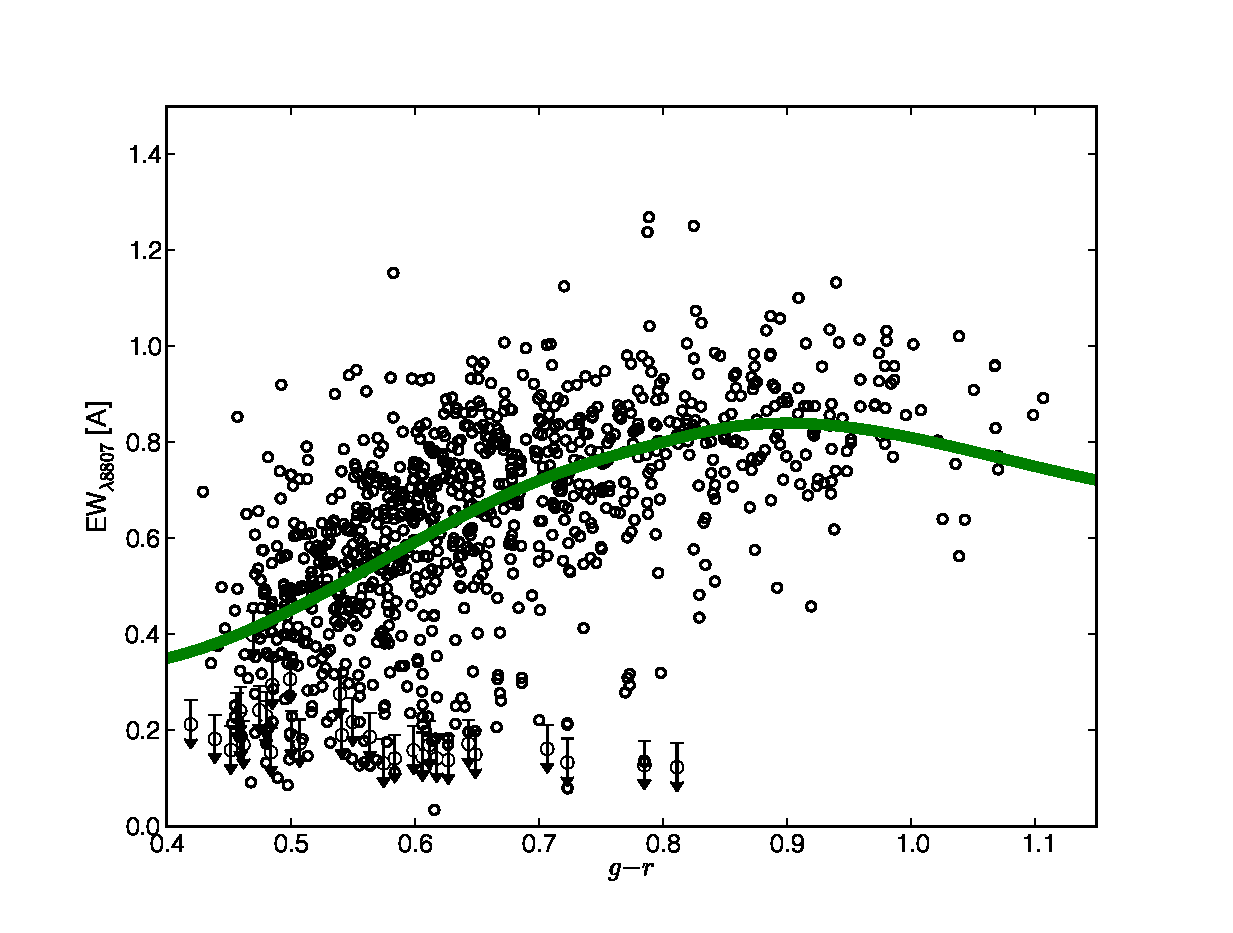
\includegraphics[width=\columnwidth]{./fig2.eps}
	\caption{SDSS $g - r$ against the measured equivalent width of the Mg\,\textsc{I} transition at 8807\,\AA{}. Dwarf contaminants occupy the more populous upper branch. Our separation line between dwarfs and giants is shown in green.}
	\label{fig:ew-mg}
\end{figure}

This dwarf/giant separation method was also employed using the total equivalent width of the Mg\,\textsc{I}\,b triplet lines. Both analyses were entirely consistent with each other: essentially the same candidate list was found using both techniques. However, given slightly poorer signal at the Mg\,\textsc{I}\,b triplet, we were forced to adopt many more upper limits than when using the 8807\,{\AA} line. Because we classify all upper limits as being ``non-dwarfs" (i.e. potential giants), we deduced a slightly larger candidate sample for the Mg\,\textsc{I}\,b analysis, which was primarily populated by upper limits. In conclusion, we found the Mg\,\textsc{I} line at 8807\,{\AA} appeared to be a more consistent dwarf discriminant given our weak S/N \--- particularly for our fainter stars. Thus, we have used the 8807\,{\AA} Mg\,\textsc{I} selection throughout the rest of our analysis.

Our dwarf/giant separation line in Figure \ref{fig:ch2-ew-mg} yields 425 potential giants. Upon taking the intersection of our kinematic and gravity selections, we find 20 stars that appear to be likely Orphan Stream giants.


\subsection{Metallicities}
\label{sec:ch2-metallicities}

We have measured the metallicities for the stars that meet our kinematic and surface gravity criteria in two ways: with the strength of their Ca\,\textsc{II} triplet lines, and by isochrone-fitting. After correcting for luminosity, the equivalent width of the Ca\,\textsc{II} triplet lines provide a good indication of the overall metallicity of a RGB star \citep{Amandroff_Da_Costa_1991}. We have employed the \citet{Starkenburg_et-al_2010} relationship and corrected for luminosity in $g$ against the horizontal branch magnitude at $g_{HB}$ = 17.1 \citep{Newberg_et-al_2010}. Strictly speaking, the Ca\,\textsc{II}\---[Fe/H] calibration is only valid for stars brighter than the horizontal branch, although the relationship only becomes significantly inappropriate near $g \-- g_{HB} \sim +1$ \citep{Saviane_et-al_2012}. Many of our candidates are fainter than this valid luminosity range, and therefore they should not be excluded solely because of their derived metallicities, as these could be uncertain. Stars fainter than $g_{HB}$ will have slightly lower metallicities than predicted by our Ca\,\textsc{II}\---[Fe/H] relationship, and for these stars we will only use metallicities to assign a relative qualitative likelihood for stream membership.

Given a distance estimate to the Orphan Stream, we can also deduce a star's metallicity through isochrone fitting. We have used a 10\,Gyr \citet{Girardi_et-al_2008} isochrone at 21.4\,kpc \citep{Newberg_et-al_2010} and found metallicities for all 20 likely stream members from their best-fitting isochrone. Derived metallicities from Ca\,\textsc{II} line strengths and isochrone fitting that are consistent (within $\pm0.3$\,dex) indicates these measurements are reliable, and that these stars are indeed at a distance of $\sim$21.4\,kpc. We find ten highly likely stream members with consistently derived metallicities. They fall within the shaded region illustrated in Figure \ref{fig:ch2-feh}. 

\begin{figure}[t!]
	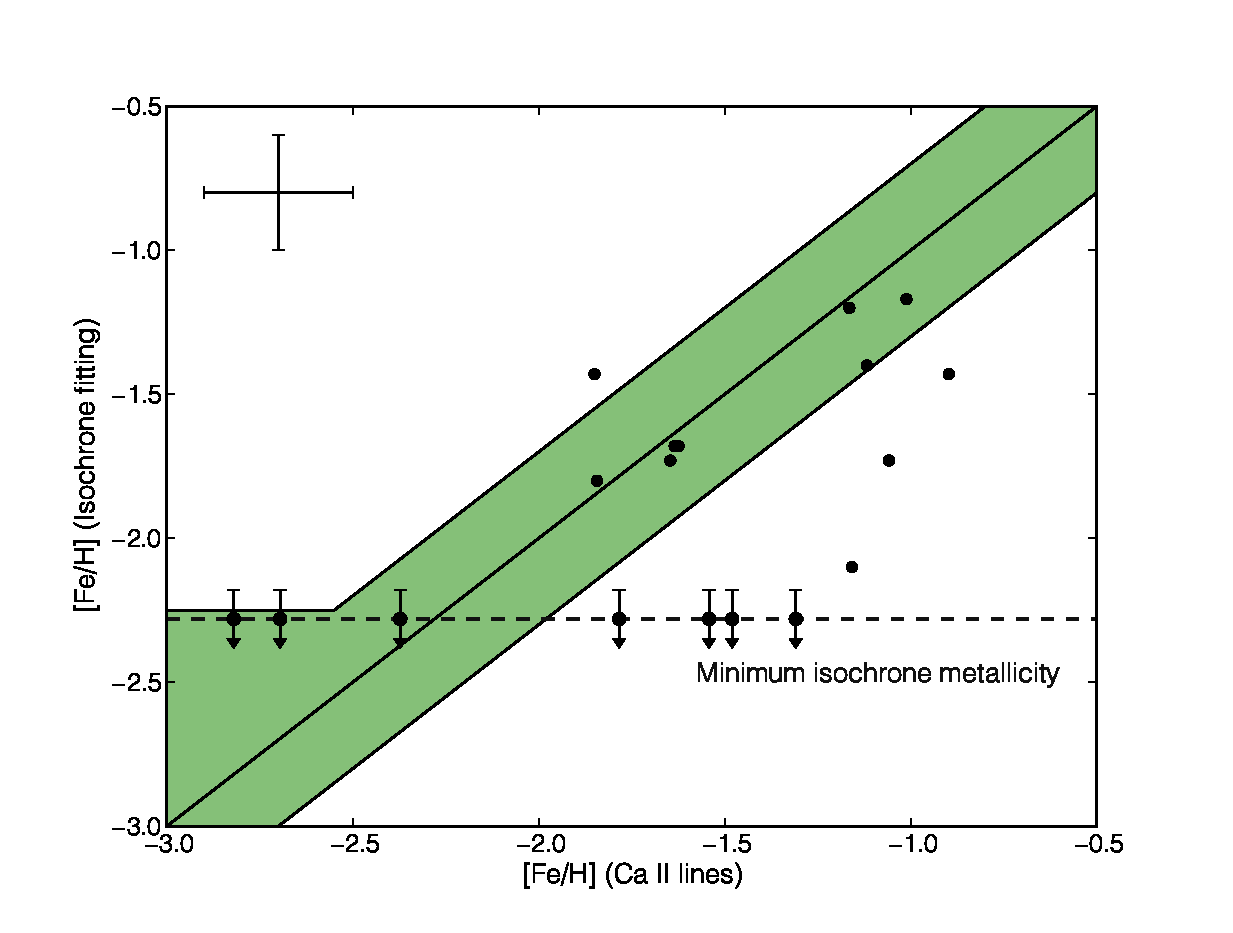
\includegraphics[width=\columnwidth]{./fig3.eps}
	\caption{Metallicities from the Ca\,\textsc{II} triplet lines versus those found from fitting isochrones to the 20 stars that meet our kinematic and surface gravity criteria. Both abundance determinations imply these stars are RGB members of the Orphan Stream at a distance of $\sim$21.4\,kpc \citep{Newberg_et-al_2010}. Consistency between these methods indicates highly likely stream membership (shaded region). The minimum isochrone [Fe/H], and a representative uncertainty of 0.2\,dex for abundance measurements is shown.}
	\label{fig:feh}
\end{figure}

\begin{figure}[t!]
	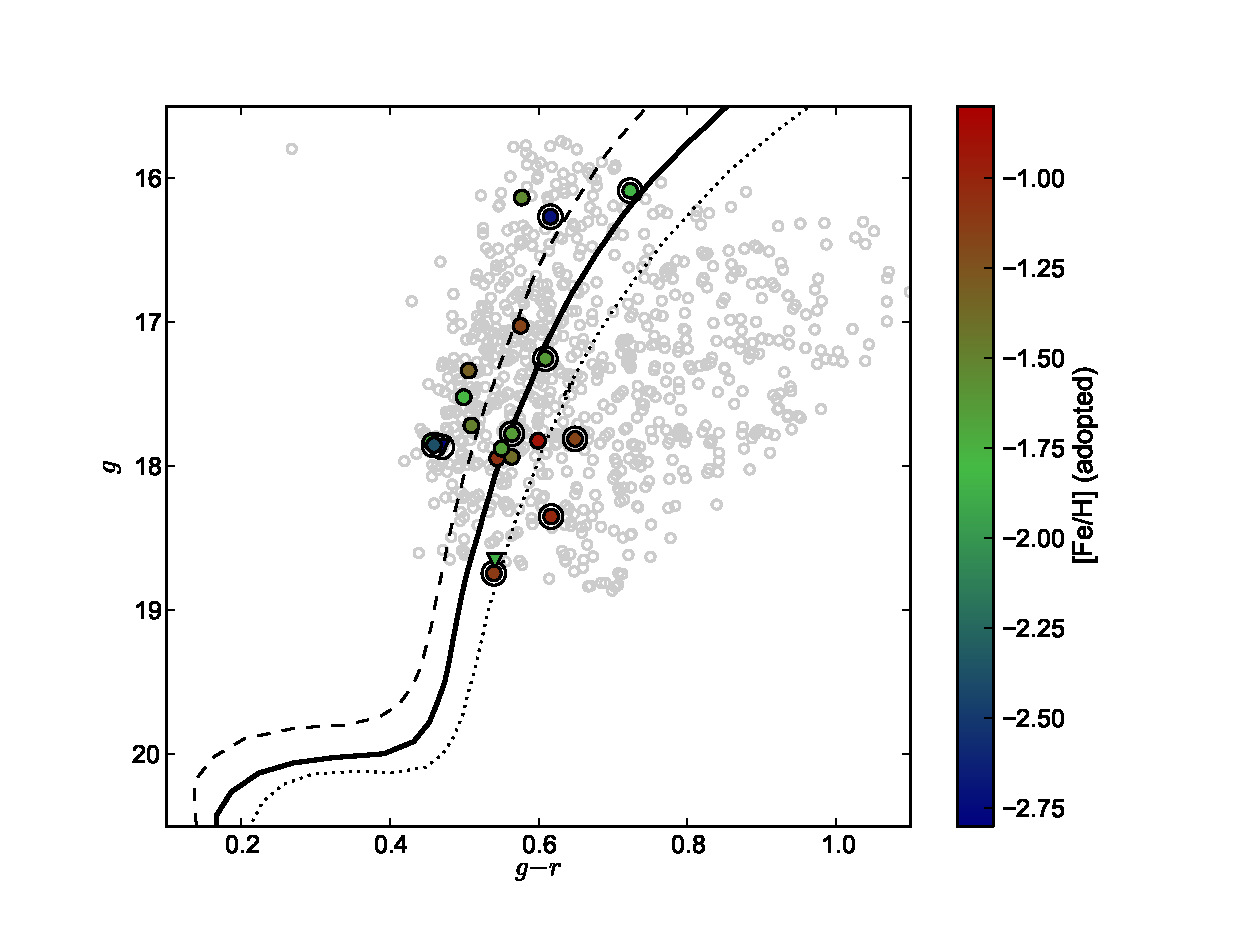
\includegraphics[width=\columnwidth]{./fig4.eps}
	\caption{Color magnitude diagram showing our observed candidates (grey). Observations fulfilling kinematic and gravity cuts are colored by their metallicity, and those with upper limits for surface gravity are marked as triangles ($\triangledown$). Highly probable stream members (see text) are circled. Relevant 10\,Gyr \citet{Girardi_et-al_2008} isochrones at $[\mbox{Fe/H}] = -1.5$ (dotted), $-2.0$ (dashed) at 21.4\,kpc \citep{Newberg_et-al_2010} are shown, as well as our best-fitting 10\,Gyr isochrone of $[\mbox{Fe/H}] = -1.63$ at 22.5\,kpc (solid).}
	\label{fig:cmd}
\end{figure}

A final metallicity value for each star has been adopted based on the quality of our [Fe/H] measurements. These values are tabulated in Table \ref{tab:oss-members}. From our highly likely stream members we find an overall stream metallicity of $[\mbox{Fe/H}] = -1.63$ with a dispersion of $\sigma = 0.56$ dex. This abundance spread is larger than typically seen in globular cluster stars and is more representative of the chemical spread seen in dSph satellites \citep[e.g.,][]{Frebel_Norris_2011}.



\setlength{\tabcolsep}{2.4pt}

\begin{table*}[t!]\footnotesize
\caption{Identified Orphan Stream Candidates\label{tab:oss-members}}
\begin{tabular*}{\textwidth}{lccccrcrcrrccccc}
\hline
\hline
Star & $\alpha$ & $\delta$ & $g$ & $g - r$ & \multicolumn{2}{c}{$\mu_\alpha$} & \multicolumn{2}{c}{$\mu_\delta$} & \multicolumn{2}{c}{$V_{GSR}$} & $EW_{\lambda8807}$ & [Fe/H]$_{Ca}$ & [Fe/H]$_{iso}$ & [Fe/H]\footnote{Final adopted [Fe/H] value based on quality of two metallicity measurements.} & Stream \\
Name & (J2000) & (J2000) & & & \multicolumn{2}{c}{(mas yr$^{-1}$)} & \multicolumn{2}{c}{(mas yr$^{-1}$)} & \multicolumn{2}{c}{(km s$^{-1}$)} & (m\AA{}) & (dex) & (dex) & (dex) & Prob. \\
\hline
OSS--1  & 10:46:21.9 & $+$00:43:21.8 & 17.52 & 0.50 & 4.1&$\pm$ 4.5 & $-$34.0 &$\pm$ 4.5 & 73.3 &$\pm$ \phn9.3 & 0.273 & --1.78 &$<$--2.28\phn\,& --1.78 & Low \\
OSS--2  & 10:46:29.3 & $-$00:19:38.5 & 17.77 & 0.56 & $-$1.7 &$\pm$ 4.3 & $-$2.2 &$\pm$ 4.3 & 78.4 &$\pm$ \phn5.2 & 0.126 & --1.63 & --1.68  & --1.63 & High \\
OSS--3  & 10:46:50.4 & $-$00:13:15.6 & 17.33 & 0.51 & 1.8 &$\pm$ 4.3 & $-$4.6 &$\pm$ 4.3 & 77.0 &$\pm$ \phn4.0 & 0.416 & --1.31 &$<$--2.28\phn\,& --1.31 & Low \\
OSS--4  & 10:47:06.1 & $-$01:56:03.9 & 18.74 & 0.54 & $-$6.3 &$\pm$ 4.9 & 4.6 &$\pm$ 4.9 & 74.9 &$\pm$    17.6 & 0.452 &:--1.12\footnote{Sufficiently fainter than $g_{HB}$ to qualify this measurement as uncertain.}& --1.40  & --1.40 & High \\
OSS--5  & 10:47:15.0 & $-$03:15:03.9 & 18.66 & 0.54 & $-$8.2 &$\pm$ 5.2 & 1.7 &$\pm$ 5.2 & 109.5 &$\pm$ \phn9.0 &$<$0.19&:--1.85\textsuperscript{b}& --1.43  & --1.43 & Medium \\
OSS--6  & 10:47:17.6 & $+$00:25:07.7 & 16.09 & 0.72 & $-$0.8 &$\pm$ 4.0 & $-$5.2 &$\pm$ 4.2 & 79.2 &$\pm$ \phn3.3 & 0.212 & --1.84 & --1.80  & --1.84 & High \\
OSS--7  & 10:47:29.1 & $-$02:02:22.6 & 17.86 & 0.47 & \multicolumn{2}{c}{\nodata} & \multicolumn{2}{c}{\nodata}  & 93.2 &$\pm$    29.8 &$<$0.40& --2.82 &$<$--2.28\phn\,& --2.82 & High \\
OSS--8  & 10:47:30.1 & $-$00:01:24.5 & 17.25 & 0.61 & $-$4.0 &$\pm$ 4.2 & $-$5.2 &$\pm$ 4.2 & 83.6 &$\pm$ \phn3.5 & 0.123 & --1.62 & --1.68  & --1.62 & High \\
OSS--9  & 10:48:20.9 & $+$00:26:34.4 & 17.88 & 0.55 & $-$8.1 &$\pm$ 4.3 & $-$5.4 &$\pm$ 4.3 & 118.9 &$\pm$    11.7 & 0.467 & --1.65 & --1.73  & --1.65 & High \\
OSS--10 & 10:48:27.8 & $+$00:55:24.0 & 17.72 & 0.51 & $-$14.4 &$\pm$ 4.6 & $-$5.3 &$\pm$ 4.6 & 124.5 &$\pm$ \phn6.7 & 0.182 & --1.48 &$<$--2.28\phn\,& --1.48 & Low \\
OSS--11 & 10:48:31.9 & $+$00:03:35.7 & 17.02 & 0.58 & $-$3.6 &$\pm$ 4.1 & $-$7.7 &$\pm$ 4.1  & 105.1 &$\pm$ \phn5.1 & 0.234 & --1.12 & --2.10  & --1.12 & Low \\
OSS--12 & 10:48:44.4 & $-$02:53:08.8 & 18.35 & 0.62 & $-$3.4 &$\pm$ 4.7 & $-$1.8 &$\pm$ 4.7 & 108.2 &$\pm$ \phn9.0 & 0.183 &:--1.01\textsuperscript{b}& --1.17  & --1.17 & High \\
OSS--13 & 10:48:46.9 & $-$00:32:27.8 & 17.85 & 0.46 & $-$28.4 &$\pm$ 4.8 & $-$12.3 &$\pm$ 4.8 & 109.3 &$\pm$ \phn8.1 & 0.324 & --2.37 &$<$--2.28\phn\,& --2.37 & Medium \\
OSS--14 & 10:49:08.3 & $+$00:02:00.2 & 16.27 & 0.62 & 4.9 &$\pm$ 4.0 & $-$6.0 &$\pm$ 4.0& 81.5 &$\pm$ \phn4.6 & 0.034 & --2.70 &$<$--2.28\phn\,& --2.70 & High \\
OSS--15 & 10:49:13.4 & $+$00:04:03.8 & 17.83 & 0.46 & 3.4 &$\pm$ 4.7 & $-$6.8 &$\pm$ 4.7 & 65.3 &$\pm$ \phn5.4 & 0.252 & --1.74 & $<$--2.28\phn\,& --1.74 & Medium \\
OSS--16 & 10:50:13.1 & $+$00:33:52.7 & 16.13 & 0.58 & $-$3.4 &$\pm$ 4.0 & $-$7.7 &$\pm$ 4.0 & 94.7 &$\pm$ \phn5.1 & 0.391 & --1.54 &$<$--2.28\phn\,& --1.54 & Low \\
OSS--17 & 10:50:24.2 & $-$01:49:05.4 & 17.94 & 0.54 & 3.4 &$\pm$ 4.6 & $-$2.2 &$\pm$ 4.6 & 109.9 &$\pm$    25.4 & 0.151 & --1.06 & --1.73  & --1.06 & Low \\
OSS--18 & 10:50:33.8 & $+$00:12:19.1 & 17.82 & 0.60 & $-$7.4 &$\pm$ 5.0 & $-$3.3 &$\pm$ 5.0 & 97.5 &$\pm$ \phn5.9 & 0.596 & --0.90 & --1.43  & --0.90 & Medium \\
OSS--19 & 10:51:19.7 & $+$00:05:15.5 & 17.81 & 0.65 & 4.2 &$\pm$ 4.7 & $-$11.8 &$\pm$ 4.7 & 82.7 &$\pm$ \phn5.0 & 0.198 & --1.16 & --1.20  & --1.16 & High \\
OSS--20 & 10:51:35.4 & $+$00:00:46.4 & 17.93 & 0.56 & --0.5 &$\pm$ 4.5 & $-$3.0 &$\pm$ 4.5 & 66.7 &$\pm$ \phn8.7 & 0.128 & :--1.38 & --2.10 & --2.10 & Medium \\

\hline
\hline
\end{tabular*}
\end{table*}



\break
\subsection{Proper Motions \& Distances}

We have found proper motions for 19 of our candidates in the PPMXL proper motion catalogue \citep{Roeser_et-al_2010}. One highly probably candidate (OSS--13 in Table \ref{tab:oss-members}) has a listed proper motion that is different from that of the other nine highly likely members at the $6\,\sigma$ level. Consequently, we have reduced the membership likelihood of this star from ``High" to ``Medium". Given the uncertainties in proper motions, we cannot reliably alter the membership probability for any other candidate.

Since our Orphan Stream giants cover a wide evolutionary range along the giant branch (Figure \ref{fig:ch2-cmd}), we are in a good position to revise the distance estimate to the stream. Given a 10\,Gyr \citet{Girardi_et-al_2008} isochrone at $[\mbox{Fe/H}] = -1.63$, we find a best-fitting distance to the stream of $22.5 \pm 2.0$\,kpc at $(l, b) = (250\,^\circ,\,50\,^\circ)$. This isochrone is shown in Figure \ref{fig:ch2-cmd}. Our derived distance is in reasonably good agreement with the measurement of $21.4 \pm 1.0$\,kpc independently deduced by \citet{Grillmair_2006} and \citet{Newberg_et-al_2010}.


\subsection{Comparison with \citet{Newberg_et-al_2010}}
\label{sec:ch2-newberg}
\citet{Newberg_et-al_2010} traced the Orphan Stream using BHB stars selected from the SEGUE survey, allowing them to derive an orbit for the stream and make a strong prediction for the location of the undiscovered progenitor. Their closest stream detection to this study is at $\Lambda_{Orphan} = 18.4\,^\circ$, approximately $\Delta\Lambda_{Orphan} \sim 4\,^\circ$ away from our fields. At this location, \citet{Newberg_et-al_2010} found the velocity of the stream to be $V_{GSR} = 101.4 \pm 8.9$\,km s$^{-1}$ based on 12 BHB stars. We note that this is $\sim95$\,km s$^{-1}$ on our scale, given the differences in accounting for the local standard of rest. The velocities and metallicities of our `High' and `Medium' probability candidates are illustrated in Figure \ref{fig:ch2-vgsr-feh}. Although we recover some candidates with velocities up to $V_{GSR} \sim 110$\,km s$^{-1}$, our kinematic distribution peaks near $V_{GSR} \sim 85$\,km s$^{-1}$, roughly 10\,km s$^{-1}$ lower than that of \citet{Newberg_et-al_2010}.

There is a known velocity gradient along the Orphan Stream which can account for this discrepancy. As $\Lambda_{Orphan}$ increases towards the edge of the SDSS boundary, galactocentric velocity quickly decreases. For the Orphan Stream detection in the outrigger SEGUE Strip 1540 at $\Lambda_{Orphan} = 36\,^\circ$, \citet{Newberg_et-al_2010} find $V_{GSR} = 38$\,km s$^{-1}$. This work presents likely Orphan Stream K-giant candidates at $\Lambda_{Orphan} \sim 23\,^\circ$. Given the velocity gradient reported by \citet{Newberg_et-al_2010}, a galactocentric velocity of $80-85$\,km s$^{-1}$ (on our scale) is perfectly reasonable. We note that since the velocities of BHB stars can have significant uncertainties, it was practical for us to assume a wide initial selection in kinematics to identify potential members. 

\begin{figure}[h!]
	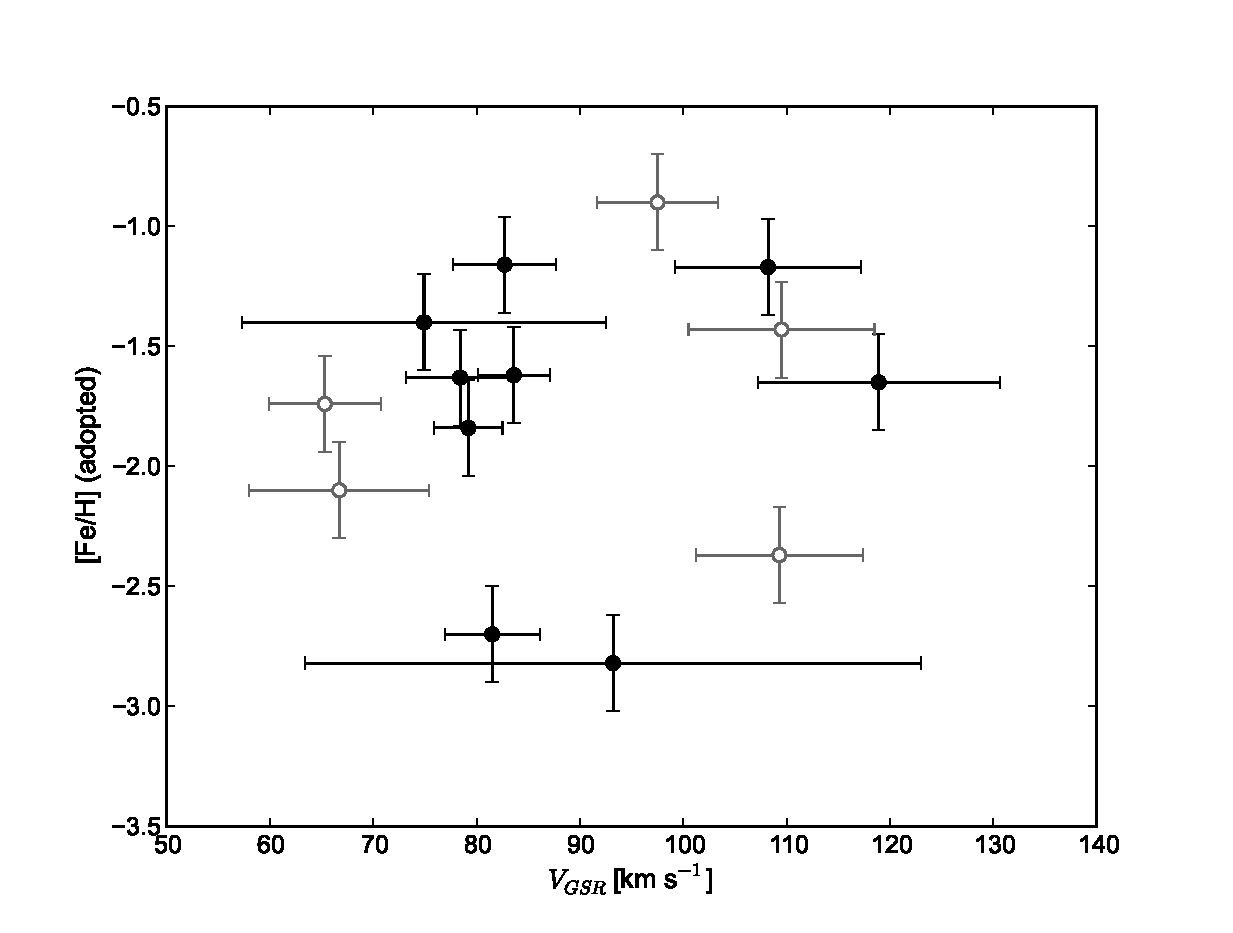
\includegraphics[width=\columnwidth]{./fig5.eps}
	\caption{Galactocentric velocities and adopted metallicities for the highest likely Orphan Stream members (black $\bullet$), and those with probabilities assigned as ``Medium'' (grey $\circ$; see text).}
	\label{fig:vgsr-feh}
\end{figure}

\begin{figure}[h!]
	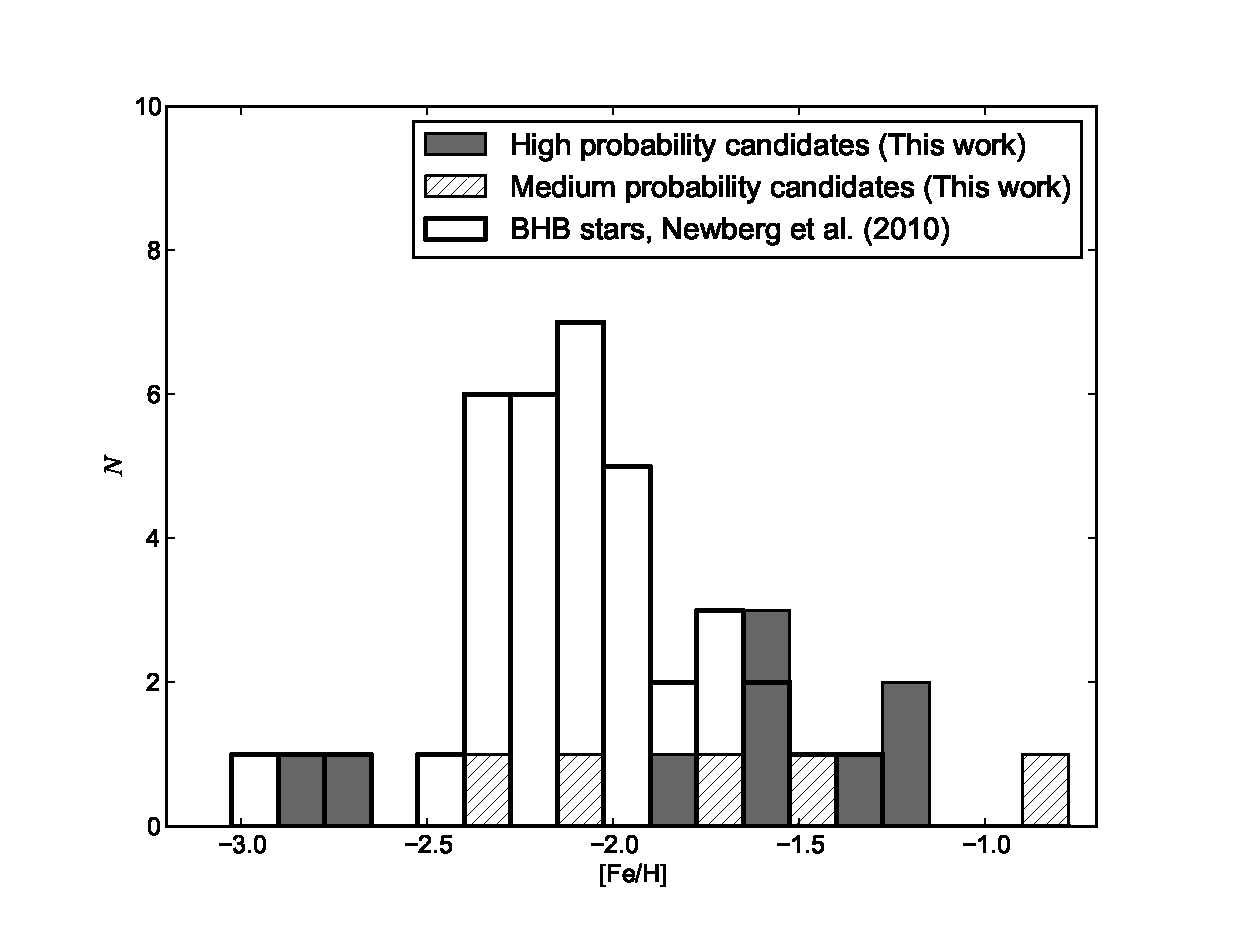
\includegraphics[width=\columnwidth]{./fig6.eps}
	\caption{Observed metallicity distribution function for the Orphan Stream candidates identified here, with comparisons to the distribution found by \citet{Newberg_et-al_2010} from BHB stars.}
	\label{fig:newberg-feh}
\end{figure}

The adopted metallicities of our Orphan Stream candidates are generally higher than those found by \citet{Newberg_et-al_2010}. Our highly likely stream members have a mean metallicity of [Fe/H] = $-1.63$, with a dispersion of $\sigma = 0.56$\,dex. As illustrated in Figures \ref{fig:ch2-vgsr-feh} and \ref{fig:ch2-newberg-feh}, there are two very metal-poor candidates which largely drive this dispersion, but we have no reason to suspect they are non-members. The \citet{Newberg_et-al_2010} sample contains 37 BHB stars identified over a 60\,$^\circ$ arc on the sky, and has a peak metallicity at [Fe/H] = $-2.10 \pm 0.10$. The closest detection bin in the \citet{Newberg_et-al_2010} sample was the most populous, yielding 7 BHB stars. For comparison, we identify 9 giant stars across $\sim{}4\,^\circ$. Given BHB stars are known to trace a somewhat more metal-poor population, and we are calculating statistics with marginal sample sizes, we conclude that the accuracy of these two metallicity distributions are not mutually exclusive. It is entirely possible that we are sampling the same distribution, but a larger sample size is required.


\section{Conclusions}
\label{sec:ch2-conclusions}

We have presented a detailed analysis to isolate individual Orphan Stream K-giants from low-resolution spectroscopy using a combination of photometric, kinematic, gravity, metallicity, and proper motion information. Although each individual criterion is likely to induce some level of contamination, their intersection reveals nine highly probable, self-consistent, Orphan Stream K-giants.  We deduce a median stream metallicity of $[\mbox{Fe/H}] = -1.63 \pm 0.19$ and find an intrinsically wide metallicity spread of $\sigma = 0.56$\,dex, indicative of a dSph origin. Unlike other stellar tracers, K-type giants can exist at all metallicities, hence our derived metallicity spread is likely representative of the true stream metallicity distribution function. Recall that the metallicity determination was performed after kinematic and gravity cuts, and three of our most probable members lay perfectly on a 10\,Gyr isochrone of $[\mbox{Fe/H}] = -1.63$. However, it is clear that more data is required to fully characterize the stream metallicity distribution function. Our data indicate a distance to the stream of $22.5 \pm 2.0$\,kpc at $(l, b) = (250\,^\circ,\,50\,^\circ)$, in agreement with that deduced by \citet{Grillmair_2006} and \citet{Newberg_et-al_2010}.

Given the stream orbit derived by \citet{Newberg_et-al_2010}, they excluded all possible known halo objects except for the dissolved star cluster, Segue 1. \citet{Simon_et-al_2011} obtained spectroscopy for six members in Segue 1 and found an extremely wide metallicity dispersion: from $<-3.4$ to $-1.63$ dex. On the basis of the extremely low metallicity in the cluster and the wide chemical dispersion, they conclude that Segue 1 is a dwarf spheroidal galaxy. Although the data presented here indicates the Orphan Stream progenitor is a disrupted dwarf spheroidal galaxy, we cannot reliably associate Segue 1 as the parent without additional observational data. 

If the Orphan Stream continues through SEGUE Stripe 1540 at $(l, b) = (271\,^\circ,\,38\,^\circ)$ as \citet{Newberg_et-al_2010} found, then the stream is even closer there than in the region analysed here. Thus, if our observations and analyses are repeated at $(271\,^\circ,\,38\,^\circ)$, we predict K-giant stream members of brighter apparent magnitude will be recovered. 

Using a maximum-likelihood estimation we find the stream velocity at $(l, b) = (250\,^\circ, 50\,^\circ)$ from nine stars to be $V_{GSR} = 85.3 \pm 4.4$\,km s$^{-1}$ and the dispersion to be $6.5 \pm 7.0$\,km s$^{-1}$. If we exclude three stars with low signal-to-noise \--- and hence large ($> 10$\,km s$^{-1}$) velocity uncertainties \--- the peak occurs at $82.1 \pm 1.4$\,km s$^{-1}$ and the intrinsic dispersion is found to be $0.2\,\pm\,3.1$\,km s$^{-1}$. Hence, the observed stream dispersion is dominated by the velocity uncertainties, indicating that the intrinsic dispersion is small. 

The K-giants presented here can provide great insight into the chemistry and history of the Orphan Stream. High-resolution spectroscopic observations have been taken for some of our highly probable members and a detailed chemical analysis will be presented in a forthcoming paper (Casey et al., in preparation). Detailed chemical abundances can help determine both the nature of the progenitor before it is discovered, and allows us to compare peculiar chemical signatures with those of the known Milky Way satellites in order to associate likely parents. However, at least for the moment, the Orphan Stream remains appropriately named.


\chapter{Conclusions}\label{conclusions}

\epigraph{Although the Universe is under no obligation to make sense, students in pursuit of the Ph.D. are.}{-- Robert P. Kirshner\footnotemark}

\footnotetext{\emph{Quarterly Journal of the Royal Astronomical Society.} 1991, Vol.\ 32, No.\ 3, p233} Lorem ipsum dolor sit amet, consectetur adipiscing elit. Duis posuere tellus eu quam pellentesque ut varius purus egestas. Nam hendrerit malesuada sapien, non molestie risus cursus at. Pellentesque habitant morbi tristique senectus et netus et malesuada fames ac turpis egestas. Sed dignissim sodales sem sed volutpat. Ut laoreet, ante sed dictum vestibulum, lacus sapien semper dui, nec rutrum velit justo eu enim. Fusce vehicula blandit ipsum, ac volutpat libero vestibulum in. Sed quis lacus mauris. Quisque congue elit in nisi lacinia ac condimentum eros pellentesque. Quisque et nisl odio, vitae eleifend neque. In volutpat sapien non leo egestas ut sodales elit malesuada. Proin suscipit, lacus a suscipit euismod, neque velit pellentesque urna, eget ullamcorper felis neque sit amet erat. Phasellus in est et ligula accumsan lacinia sit amet et nisl. Aliquam interdum, arcu sed dictum gravida, mi justo iaculis mi, vel scelerisque nulla nunc in justo \citep{Murphy12}.

Phasellus erat libero, lobortis vitae iaculis nec, congue et tortor. Donec tempus leo et nisl tincidunt porta. Nulla velit sapien, sollicitudin sit amet accumsan a, facilisis a est. Phasellus scelerisque convallis sapien, nec viverra dui tincidunt a. Nulla ligula velit, laoreet fringilla condimentum sed, euismod a est. Fusce leo sapien, rhoncus a ultricies nec, porttitor ut lectus. Sed vestibulum turpis risus, nec vestibulum diam. Morbi quis quam quis enim cursus aliquam scelerisque quis tellus. Pellentesque accumsan lectus cursus massa ultrices placerat. Nulla facilisi. Praesent fermentum erat in augue sagittis condimentum. Nullam posuere blandit urna a mollis. Cras malesuada lectus a turpis sollicitudin volutpat. Morbi semper, nisl vel mattis vehicula, sapien sapien adipiscing tortor, in accumsan tortor dolor non neque. Maecenas varius, nunc ut euismod volutpat, mauris ante faucibus magna, ac eleifend elit tortor sed arcu.

\section{Future prospects} 

Lorem ipsum dolor sit amet, consectetur adipiscing elit. Duis posuere tellus eu quam pellentesque ut varius purus egestas. Nam hendrerit malesuada sapien, non molestie risus cursus at. Pellentesque habitant morbi tristique senectus et netus et malesuada fames ac turpis egestas. Sed dignissim sodales sem sed volutpat. 

\subsection{What you were going to do in your Ph.D.}

Ut laoreet, ante sed dictum vestibulum, lacus sapien semper dui, nec rutrum velit justo eu enim. Fusce vehicula blandit ipsum, ac volutpat libero vestibulum in. Sed quis lacus mauris. Quisque congue elit in nisi lacinia ac condimentum eros pellentesque. Quisque et nisl odio, vitae eleifend neque. In volutpat sapien non leo egestas ut sodales elit malesuada. Proin suscipit, lacus a suscipit euismod, neque velit pellentesque urna, eget ullamcorper felis neque sit amet erat. Phasellus in est et ligula accumsan lacinia sit amet et nisl. Aliquam interdum, arcu sed dictum gravida, mi justo iaculis mi, vel scelerisque nulla nunc in justo.

Phasellus erat libero, lobortis vitae iaculis nec, congue et tortor. Donec tempus leo et nisl tincidunt porta. Nulla velit sapien, sollicitudin sit amet accumsan a, facilisis a est. Phasellus scelerisque convallis sapien, nec viverra dui tincidunt a. Nulla ligula velit, laoreet fringilla condimentum sed, euismod a est. Fusce leo sapien, rhoncus a ultricies nec, porttitor ut lectus. Sed vestibulum turpis risus, nec vestibulum diam. Morbi quis quam quis enim cursus aliquam scelerisque quis tellus. Pellentesque accumsan lectus cursus massa ultrices placerat. Nulla facilisi. Praesent fermentum erat in augue sagittis condimentum. Nullam posuere blandit urna a mollis. Cras malesuada lectus a turpis sollicitudin volutpat. Morbi semper, nisl vel mattis vehicula, sapien sapien adipiscing tortor, in accumsan tortor dolor non neque. Maecenas varius, nunc ut euismod volutpat, mauris ante faucibus magna, ac eleifend elit tortor sed arcu.


\subsection{Save some work for your first post-doc}

Vestibulum sed orci nec diam euismod vehicula vitae et mauris. Phasellus sagittis justo quis mauris adipiscing auctor. Suspendisse nibh erat, cursus vitae aliquam in, rutrum sed est. Nunc mollis quam quis velit vehicula fringilla. Quisque convallis, neque ut faucibus luctus, nisl ante porttitor ante, at venenatis lectus nulla sed augue. Quisque lacinia semper lacus, nec ultricies justo auctor vel. Aenean viverra aliquam est ac porttitor.

Aliquam egestas elementum enim, id porta libero sodales ac. Fusce mattis ultrices tortor, eget iaculis nibh ultrices et. Fusce eget ligula quam. Vivamus id nisi non sapien venenatis adipiscing. Mauris posuere imperdiet elit, vitae accumsan nibh vehicula eget. Curabitur et magna mi, vel elementum velit. Class aptent taciti sociosqu ad litora torquent per conubia nostra, per inceptos himenaeos. Donec placerat arcu eget eros ornare viverra.



%
%%% BACK CONTENT:
%
\cleardoublepage
% for back matter, plain page style with no head/foot rules
%\pagestyle{plain}

%
% bibliography
\phantomsection\addcontentsline{toc}{chapter}{Bibliography}
% change bib style to 'apj' to remove the ADS links in the printed version
\bibliographystyle{astroads}
\bibliography{references}

% appendices
\cleardoublepage
 \phantomsection
 %
 % I like my appendices to just follow on  from the main text,
 % without a fresh title page
 %
%\appendix
%\appendixpage
%\addappheadtotoc
\begin{appendices}
\chapter{An image of a kitten}

A kitten is a juvenile domesticated cat. A feline litter usually consists of two to five kittens. To survive, kittens need the care of their mother for the first several weeks of their life. Kittens are highly social animals and spend most of their waking hours playing and interacting with available companions. The word \emph{``kitten''} derives from Middle English \emph{kitoun} (ketoun, kyton etc.), which itself came from Old French \emph{chitoun}. The young of big cats are called cubs rather than kittens. Either term may be used for the young of smaller wild felids such as ocelots, caracals, and lynx, but \emph{kitten} is usually more common for these species.

\begin{figure}[b!] 
   \centering
   
\includegraphics[width=0.9\textwidth]{kitten.jpg} 
   \caption{The aforementioned kitten}
   \label{fig:kitten}
\end{figure}

\chapter{Lots of awful mathematics}
\vspace{-1cm}\emph{\small We follow the standard derivation of \citet{Murphy12b}. This differs from that used by \cite{Murphy12}, who follow \citet{Murphy11} in using Lindblad's original approach. \citet{Murphy10} derive the approximation in heliocentric coordinates in terms of the initial $XYZ$ position and $UVW$ velocity of the test particle. The two derivations are equivalent, as are the standard angular frequencies $\Omega$, $\kappa$ and $\nu$.}\\

We first assume a gravitational potential for the Galactic disk $\Phi$ that is axisymmetric around the normal to the disk. We also assume that such a potential is symmetric about the disk plane. In cylindrical $(R,\phi,z)$ coordinates the equations of motion for such a potential are:
\begin{align}\label{eqn:eom}
\begin{split}
\ddot{R}-R\dot{\phi}^2& = -\frac{\partial \Phi}{\partial R} \\
\frac{d}{dt}(R^{2}\dot{\phi})& = 0 \\
\ddot{z}&=-\frac{\partial\Phi}{\partial z}
\end{split}
\end{align}
Noting that the second equation implies the conservation of angular momentum about the $z$ axis; $R^{2}\dot{\phi}=\textrm{constant} = L_{z}$, the equations of motion can also be written
\begin{align}\label{eqn:eqnmotion}
\begin{split}
\ddot{R} = -\frac{\partial \Phi_{\rm eff}}{\partial R} \quad\textrm{and}\quad \ddot{z} = -\frac{\partial \Phi_{\rm eff}}{\partial z} 
\end{split}
\end{align}
where the effective potential $\Phi_{\rm eff}(R,z)$ is defined as
\begin{align}
\Phi_{\rm eff}(R,z) = \Phi(R,z) + \frac{L_{z}^{2}}{2R^{2}}
\end{align}
The effective potential has a minimum at $z=0$ (by symmetry) and at $R=R_{g}$:
\begin{align}
\frac{\partial \Phi_{\rm eff}}{\partial R} = \frac{\partial \Phi}{\partial R} - \frac{L_{z}^{2}}{R^{3}} = 0 \quad\textrm{which means}\quad \frac{\partial \Phi}{\partial R}\bigg|_{(R_{g},0)} = \frac{L_{z}^{2}}{R_{g}^{3}} = R_{g}\dot{\phi}^{2}
\end{align}
The \emph{guiding centre} radius $R_{g}$ therefore corresponds to a circular orbit with constant angular speed $\dot{\phi}=\Omega_{g}=\sqrt{(1/R)\partial \Phi/\partial R}=L_{z}/R_{g}^{2}$. We can approximate the effective potential around $(R,z)=(R_{g},0)$ by the second-order Taylor expansion around this point. If we define $x=(R-R_{g})$ the expansion is:
\begin{align}
\begin{split}
\Phi_{\rm eff} &\simeq \Phi_{\rm eff}(R_{g},0) + x\frac{\partial\Phi_{\rm eff}}{\partial R}\bigg|_{(R_{g},0)} + z\frac{\partial\Phi_{\rm eff}}{\partial z}\bigg|_{(R_{g},0)}\\
&+ \frac{1}{2}x^{2}\frac{\partial^{2}\Phi_{\rm eff}}{\partial R^{2}}\bigg|_{(R_{g},0)} + \frac{1}{2}z^{2}\frac{\partial^{2}\Phi_{\rm eff}}{\partial z^{2}}\bigg|_{(R_{g},0)} + xz\frac{\partial^{2}\Phi_{\rm eff}}{\partial R\partial z}\bigg|_{(R_{g},0)} 
\end{split}
\end{align}
The second and third terms are zero at the point $(R_{g},0)$. The cross-term is also zero as we assume the potential is symmetric about $z=0$. The effective potential then becomes
\begin{align}
\begin{split}
\Phi_{\rm eff} &\simeq \Phi_{\rm eff}(R_{g},0) + \frac{1}{2}x^{2}\frac{\partial^{2}\Phi_{\rm eff}}{\partial R^{2}}\bigg|_{(R_{g},0)} + \frac{1}{2}z^{2}\frac{\partial^{2}\Phi_{\rm eff}}{\partial z^{2}}\bigg|_{(R_{g},0)}\\
&= \Phi_{\rm eff}(R_{g},0) + \frac{1}{2}(\kappa x)^{2} + \frac{1}{2}(\nu z)^{2}
\end{split}
\end{align}
where we define the constants:
\begin{align} 
\kappa^{2} = \frac{\partial^{2} \Phi_{\rm eff}}{\partial R^2}\bigg|_{(R_{g},0)} \quad\textrm{and}\quad \nu^{2} = \frac{\partial^{2} \Phi_{\rm eff}}{\partial z^2}\bigg|_{(R_{g},0)}
\end{align}
In this second-order Taylor expansion of the effective potential the equations of motion (Eqn. \ref{eqn:eqnmotion}) simplify to those of harmonic oscillators:
\begin{align}\label{eqn:harmonic}
\ddot{x} = -\kappa^{2} x \quad\textrm{and}\quad \ddot{z} = -\nu^{2} z
\end{align}
which have the general solutions:
\begin{align}\label{eqn:xz}
x(t) = X\cos(\kappa t + \alpha)\quad \textrm{and}\quad z(t) = Z\cos(\nu t + \beta)
\end{align}
for constants $X,Z,\alpha$ and $\beta$. What about the azimuthal coordinate $\phi$? Realising that angular momentum is conserved and $\dot{\phi}=L_{z}/R^{2}$ and $\Omega_{g}=L_{z}/R_{g}^{2}$, we have
\begin{align}
\dot{\phi} = \frac{L_{z}}{R_{g}^{2}}\frac{1}{(x/R_{g}+1)^{2}} \simeq \Omega_{g}\bigg(1-2\frac{x}{R_{g}}\bigg)
\end{align}
Substituting for $x(t)$ and integrating we arrive at
\begin{align}
\phi = \Omega_{g} t -2\frac{\Omega_{g}}{R_{g}\kappa}X\sin(\kappa t + \alpha) + \phi_{0}
\end{align}
If we convert the cylindrical $(R,\phi,z)$ coordinate system to a Cartesian system $(x,y,z)$, comoving with the guiding centre $(R_{g},\phi$); for $X \ll R_{g}$ this simplifies to:
\begin{align}
\begin{split}\label{eqn:y}
y(t) &= -2\frac{\Omega_{g}}{\kappa} X\sin(\kappa t + \alpha) \\
&= -Y\sin(\kappa t + \alpha)
\end{split}
\end{align}
In the new coordinate system $x$ and $z$ are the same as above and $y$ points in the direction of Galactic rotation. In this frame the star can  be thought of as simultaneously oscillating around the guiding centre vertically and in an ellipse in the $xy$ plane (the epicycle). The motion can be described by three angular frequencies; the epicyclic frequency $\kappa$, the vertical frequency $\nu$ and the angular velocity of the guiding centre, $\Omega_{g}$.  The vertical motion is independent of the epicyclic motion. The size of the epicycle is dictated by the ratio of $\kappa$ to $\Omega_{g}$: $X/Y = \kappa/2\Omega_{g}$.  The resultant orbital motion following Equations~\ref{eqn:xz} and \ref{eqn:y} in a Galactocentric inertial frame is traced in Figure~\ref{fig:orbit}. Like in the general case, although close to circular, the orbit is not closed in such a frame.

\begin{figure}[p!] 
\vspace{-2mm}
   \centering
   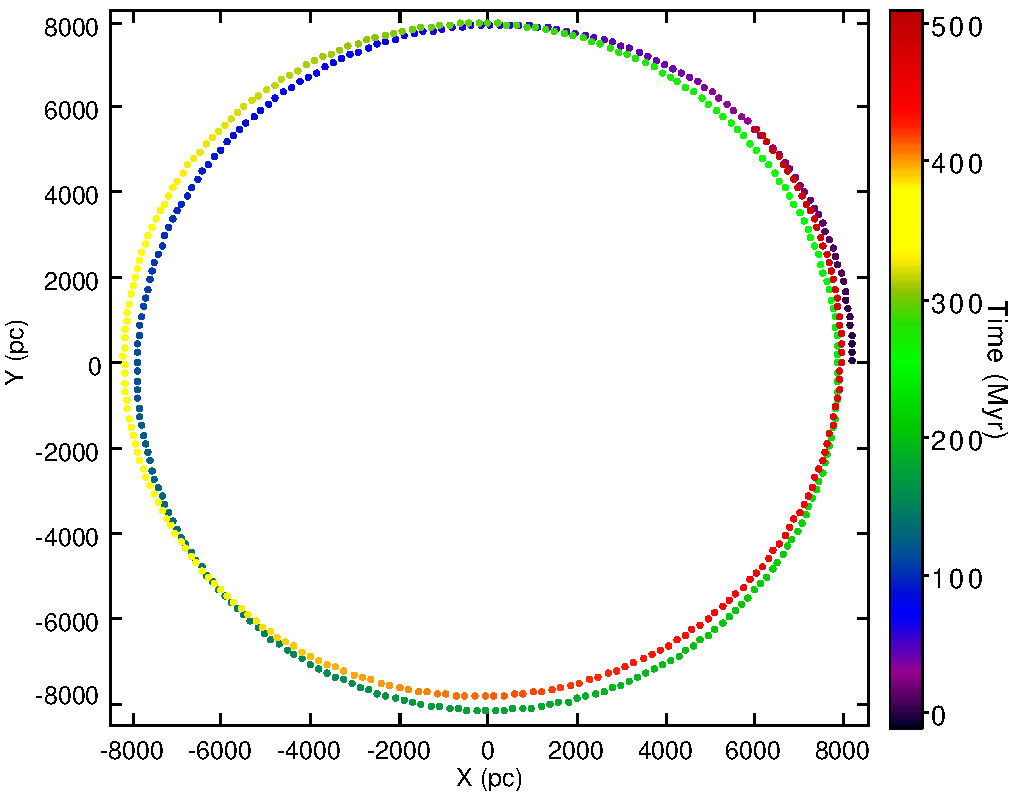
\includegraphics[width=0.68\textwidth]{orbit_xy}\\ 
   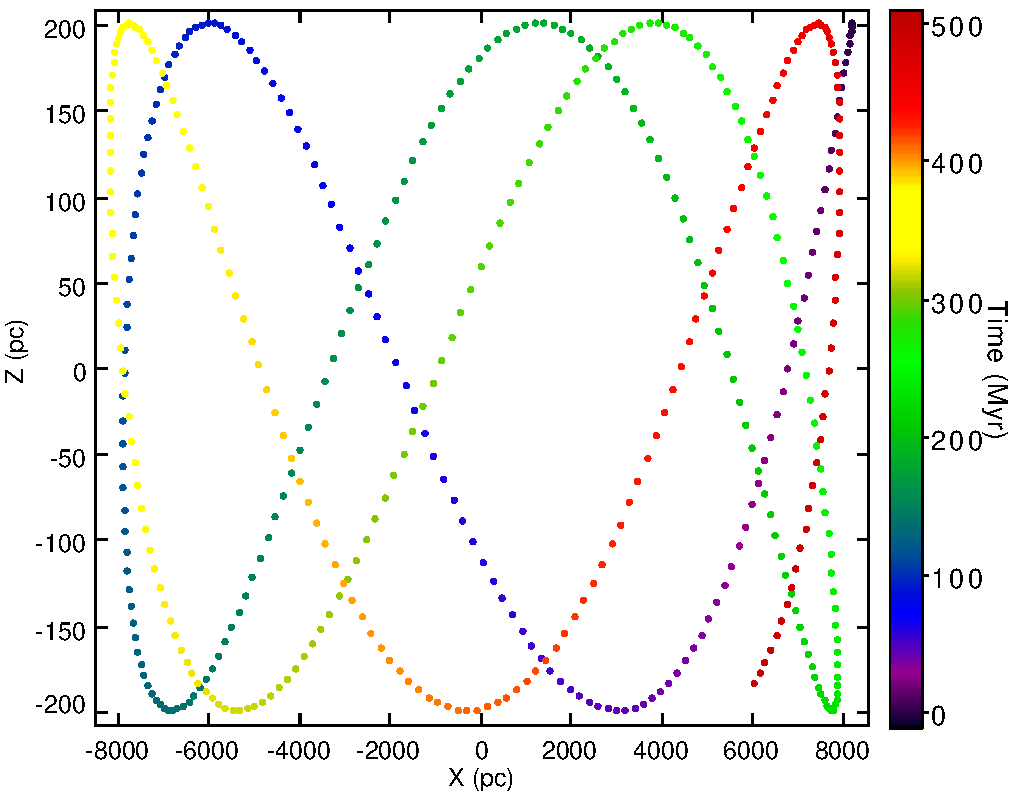
\includegraphics[width=0.68\textwidth]{orbit_xz}\\
   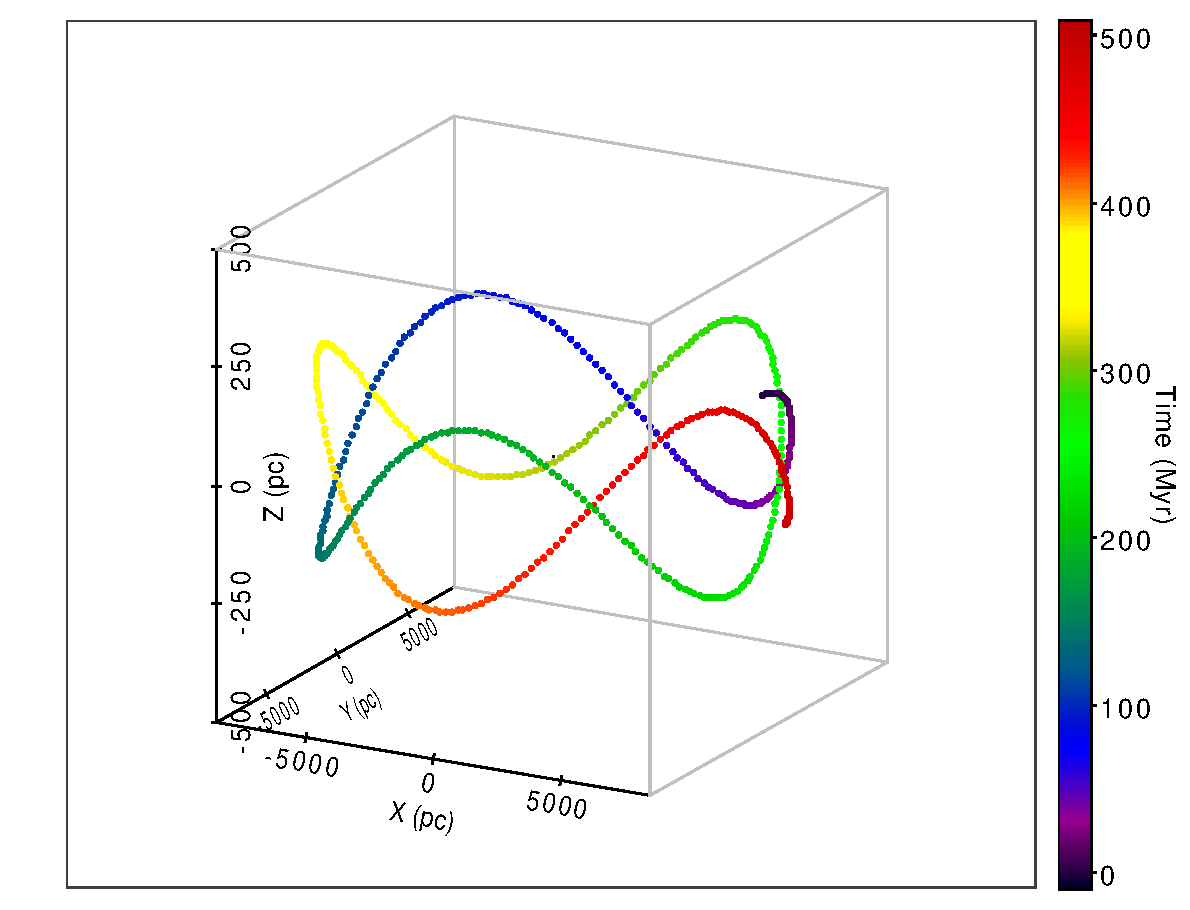
\includegraphics[width=0.68\textwidth]{orbit_xyz} 
   \caption[Orbital motion in the epicyclic approximation]{Orbital motion  with $\kappa_{0}=0.0367$~\kms~pc$^{-1}$ , $\Omega_{0}=0.0272$~\kms~pc$^{-1}$, $R_{g}=R_{\odot}=8000$~pc and $X=Z=200$~pc. The coordinate system has its origin at the Galactic centre.}
   \label{fig:orbit}
\end{figure}




\end{appendices}
\end{document}
